\section{Personal Contribution}
\label{Appendix:Contribution}

\subsection{Contribution to $ZZ(\rightarrow 4\ell)jj$ Measurement} 
\label{subsec:ZZjjContr}

The measurement presented in this thesis is only possible from the effort of the entire analysis team. I am one of the two primary analyzers who have contributed to several measurement areas from its initial formation to the current stage of finalization and publication. I contributed significantly to defining the analysis phase space discussed in Chapter $IV$. The phase space defined in the preceding ATLAS analysis \cite{ATLASZZjj}, which observed the electroweak $ZZjj$ process was not optimal for differential measurement. Therefore, I worked on loosening the kinematic selections to increase the acceptance, defining the isolation working point to maintain optimal signal-selection and background-rejection probabilities, and establishing novel pair sorting strategy to reduce the bin migration in unfolding. Moreover, I was responsible for maintaining the main analysis framework, which implements the latest recommendations from combined performance groups for physics object reconstruction discussed in Chapter $III$, and applies most of the kinematic cuts for object and event selection discussed in Chapter $IV$. This framework applies all the scale factors and event weights in MC events, and selects a few hundred relevant physics events that passes all kinematic selections for both data and MC. Additionally, I estimated the fake backgrounds of the analysis using the background estimation technique discussed in Section \ref{sec:Bkg} and assisted in selecting relevant systematics discussed in Section \ref{sec:Uncertainties} of Chapter $V$. I also validated the novel next-to-leading-order \textsc{Powheg} $qqZZjj$ MC sample used as the primary sample for the electroweak production of $ZZ(\rightarrow 4\ell)jj$. 

\subsection{Contribution to the ATLAS Experiment}
\label{subsec:ATLASContr}
I have been a member of the ATLAS collaboration since $2017$ and have contributed to the three critical areas of the experiment; detector development, detector performance, and physics analyses.

\textbf{Detector Developement:}
I spent my first year as a graduate student working at Brookhaven National Lab, where I contributed to the prototype development of the all-silicon inner tracker for the high luminosity LHC. During this period, I assembled the first three prototype staves, the detector units of the ITk strip barrel region detector, using a semi-automated loading setup consisting of an Aeoretch robotic arm, cameras, and an alignment system. I developed a $3D$-printed tooling pins used in the alignment of loading the sensors on staves. I led comprehensive thermal and mechanical tests of the first prototype, the thermo-mechanical stave using IR imaging and laser metrology, respectively. These tests validated the cooling system designs of the ITk stave core structure and the stability of the mechanical design, giving the green light to the production of $200$ out of $400$ strip-staves needed to build the barrel region of the inner tracker. During this year, I learned the fundamentals of particle physics detectors, their development, and their operations.  

\textbf{Physics Analysis:}
Apart from the $ZZ(\rightarrow 4\ell)jj$ analysis presented in this thesis, I have worked on two other ATLAS analyses involving four leptons in the final state, analyzing the complete Run-2 datasets. After my Ph.D. candidacy and ATLAS qualification, I joined the inclusive four-lepton measurement analysis team, whose goal was to inclusively measure the unfolded cross-sections of the Standard Model four-lepton process. In a year as a part of the team, I worked on finding the suitable lepton isolation working points, studying the impact of including electrons and muons originating from tau leptons in the unfolded differential cross-sections, and the most precise measurement to date of the branching ratio of $ Z \to 4\ell$ with full Run-2 dataset.

Since early 2021, I have been a crucial part of the on-shell $ZZ$ CP and polarization analysis team, where the main goal is to extract the fraction of two $Z$ bosons simultaneously longitudinally polarized and search for additional CP violation. Like the $ZZ(\rightarrow 4\ell)jj$ analysis, I have contributed to background estimation, phase space optimization, and event selection. Additionally, I have contributed to deriving the unfolded cross-sections with all relevant systematic and statistical uncertainties used in CP violation searches using an effective field theory approach. 

\textbf{Detector Performance: }
The training of a particle physicist is incomplete without understanding the detector's performance. Therefore, in 2021 I joined the Tracking Combined Performance group of ATLAS and have contributed to the validation of the performance of the Run-3 tracking reconstruction software in both early Run-3 data and different types of MC simulation. 

Similar to $ZZ(\rightarrow 4\ell)jj$ measurement, most ATLAS physics analyses use the vertex with the highest value of the sum-squared of track's transverse momenta $(\sum_{tracks}{p_{T}^2})$ as the hard scattering vertex of the measurement. However, in processes with softer leptons and invisible tracks (including photons), $\sum_{tracks}{p_{T}^2}$ is inadequate to identify the hard scatter vertex. Therefore, I am currently working on developing an alternative algorithm that is suitable for a variety of different physics processes. 

The experience I have gained in different areas of particle physics has significantly shaped my discussion of the measurement presented in this document.  

\section{Additional Study on Unfolding Bias}
\label{Appendix:Unfolding_bias}
As discussed in Section \ref{subsec:Bias}, the bias from the unfolding process is the largest source of the systematic uncertainty for the measurement. Additional studies were conducted to understand the underlying source of this bias. Figure \ref{fig:UnfoldingBiasStat_mjj_VBSEnhanced} shows the unfolding bias and statistical uncertainty on the unfolded yield as a function of the increasing number of unfolding iterations for each bin of $m_{jj}$ in the VBS-Enhanced region. The bias is evaluated using the MC-toy-based method introduced in Section \ref{subsec:Bias}. The total uncertainty shown in the black distribution is always the smallest for a single iteration, further assuring the choice of iteration is optimal. As expected, the bias decreases and the statistical uncertainty increases with the increasing number of unfolding iterations.

\begin{figure}[htb]
    \centering
    \begin{subfigure}{.48\textwidth}
        \centering
        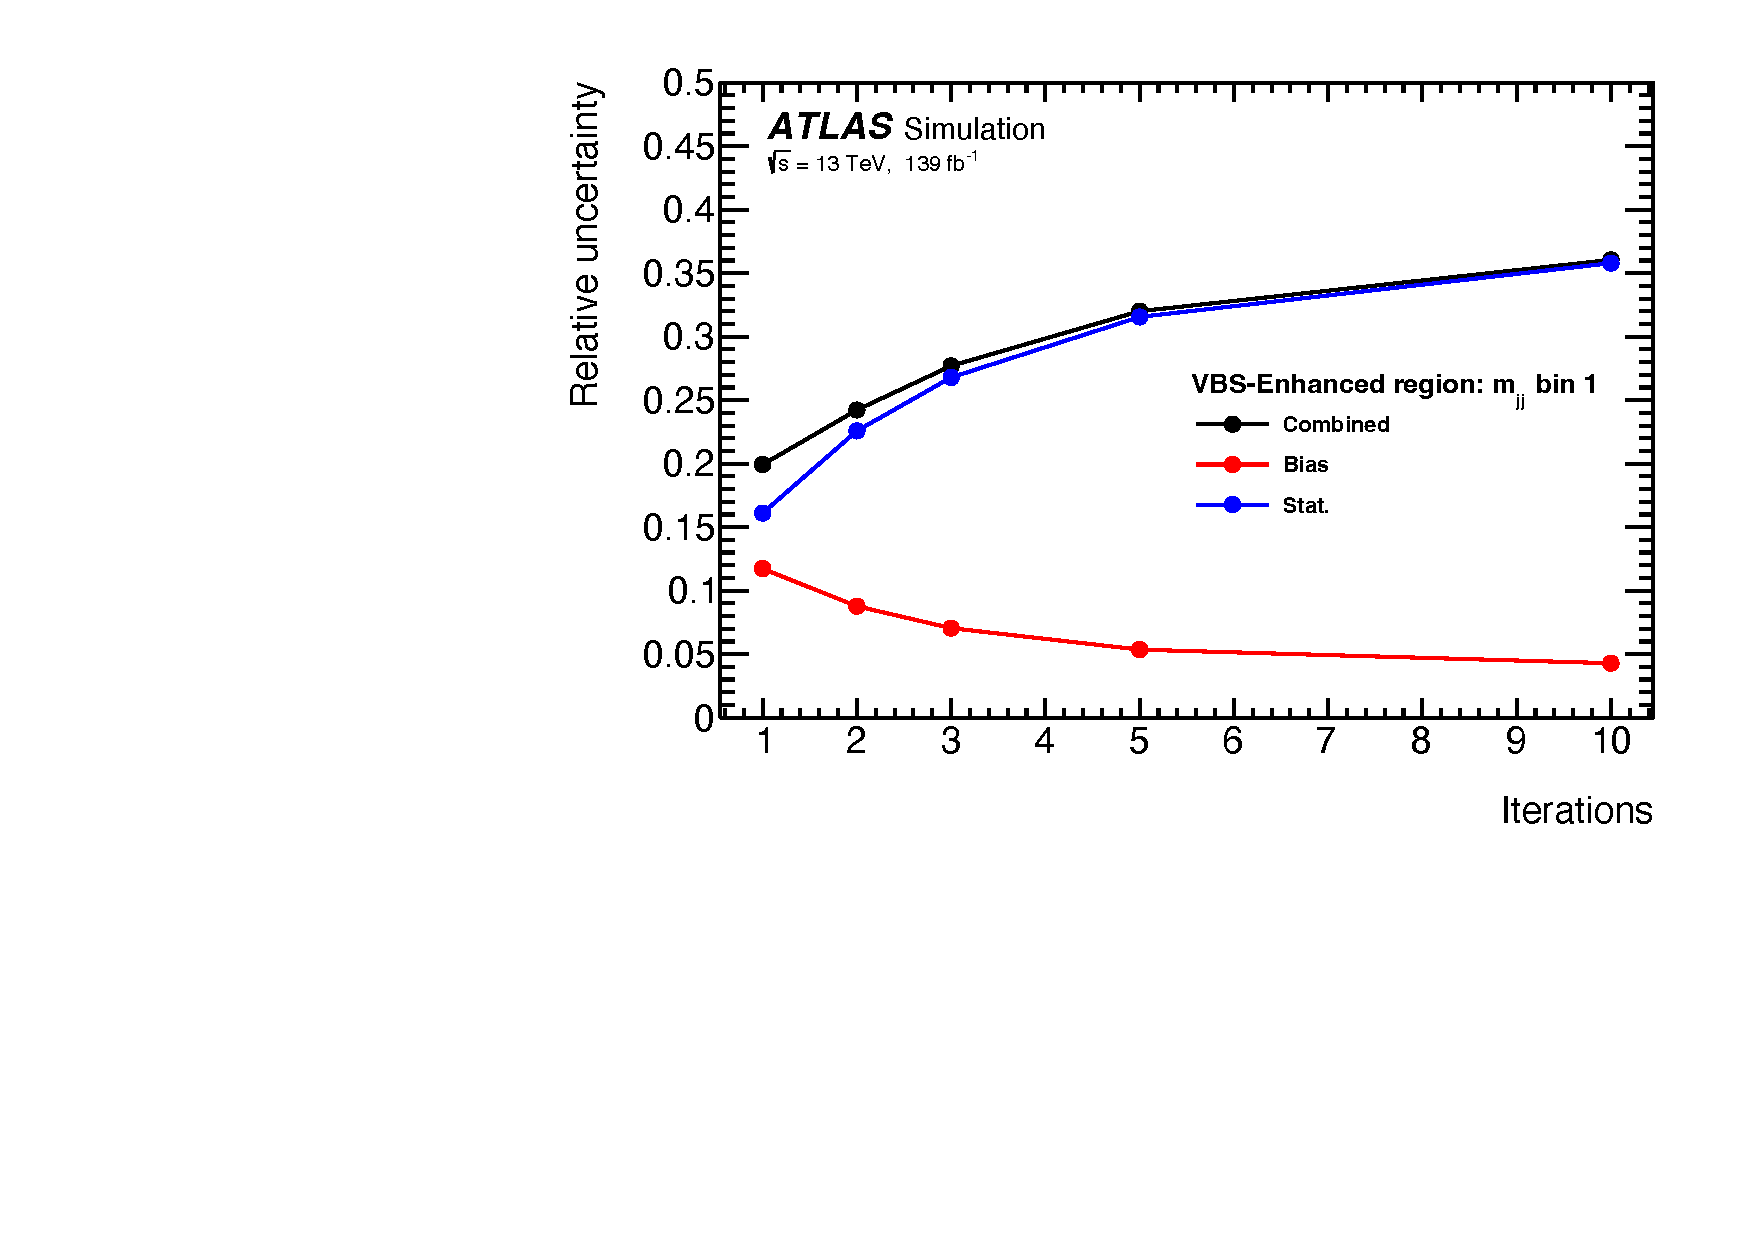
\includegraphics[width=.9\linewidth]{figures/Analysis/Unfolding/unfoldingbias/unfolding_bias_stat_unc_mjj_VBSEnh_bin1.pdf}
        \caption{ bin 1}
    \end{subfigure}
    \begin{subfigure}{.48\textwidth}
        \centering
        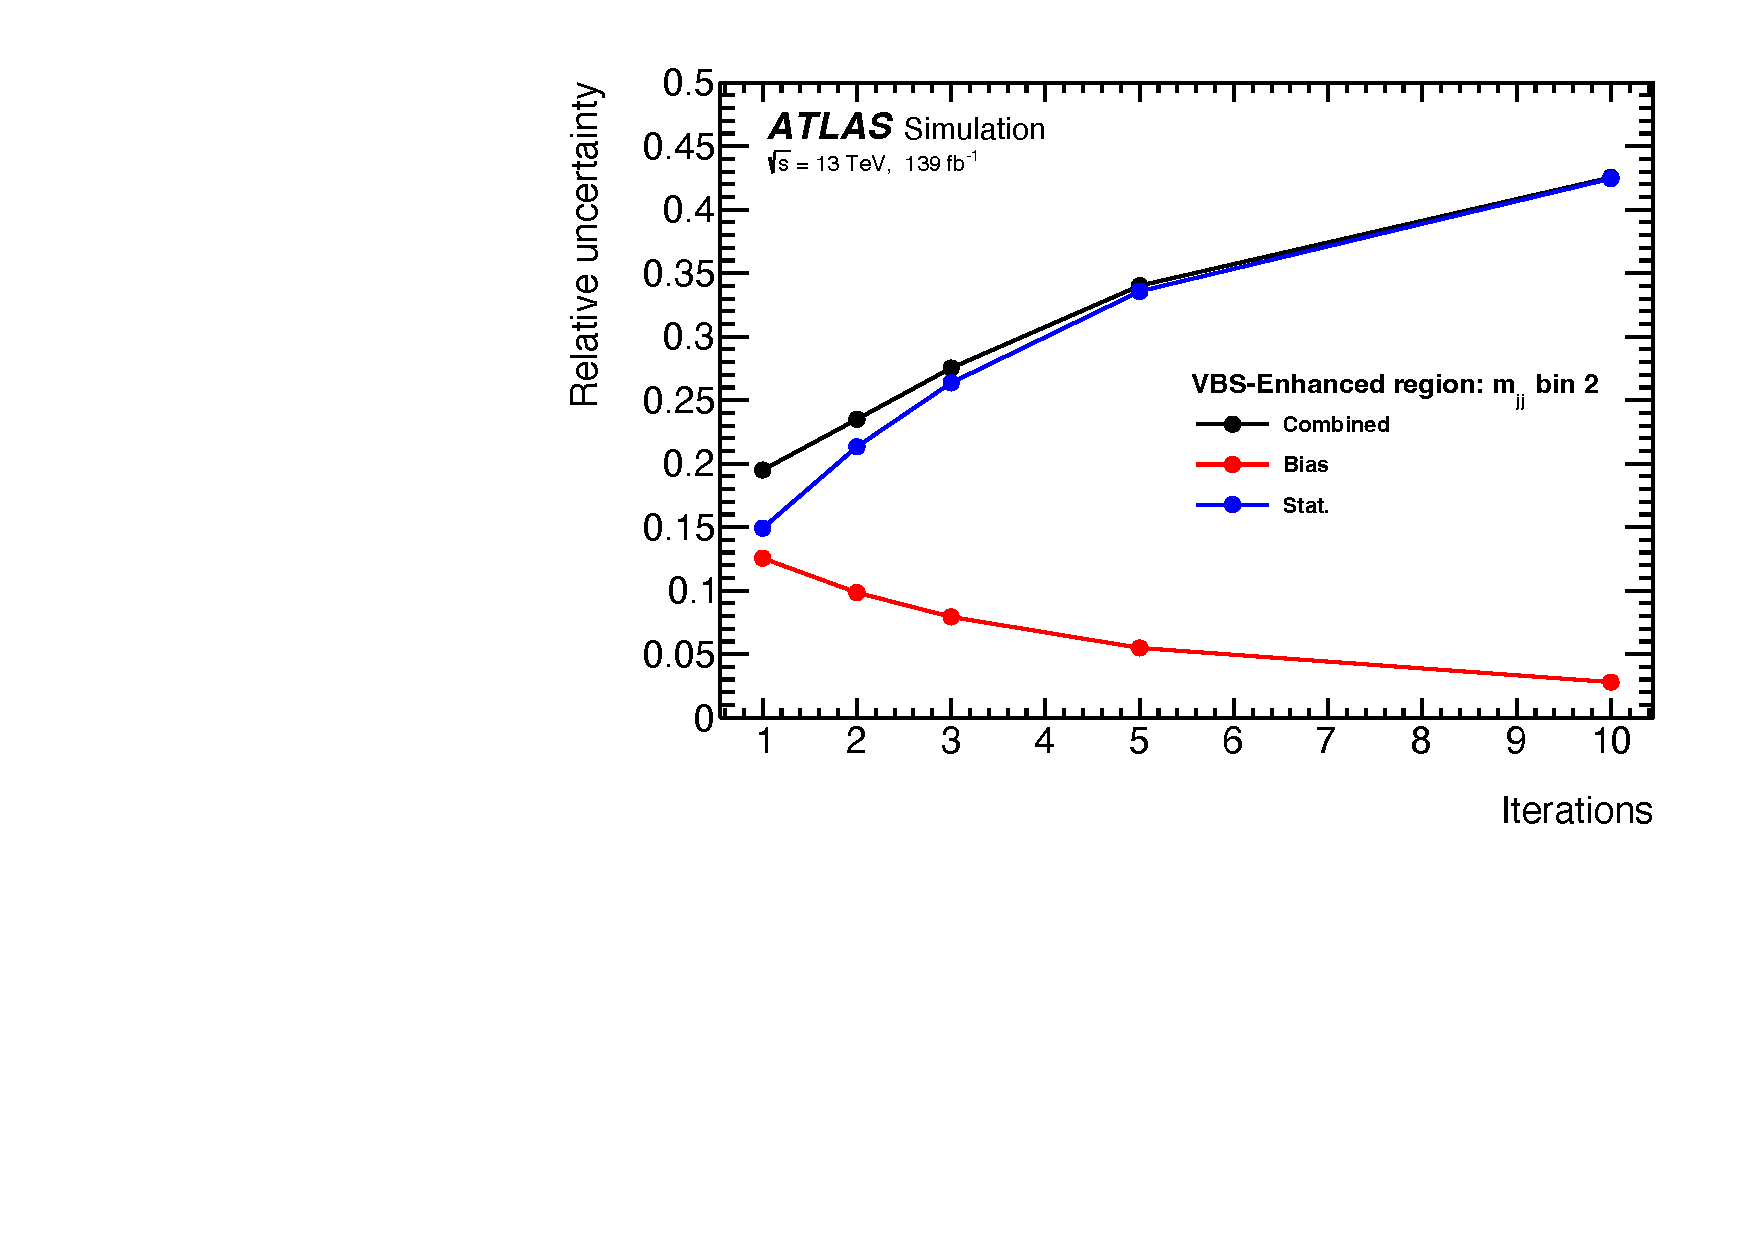
\includegraphics[width=.9\linewidth]{figures/Analysis/Unfolding/unfoldingbias/unfolding_bias_stat_unc_mjj_VBSEnh_bin2.pdf}
        \caption{bin 2 }
    \end{subfigure}\\
    \begin{subfigure}{.48\textwidth}
        \centering
        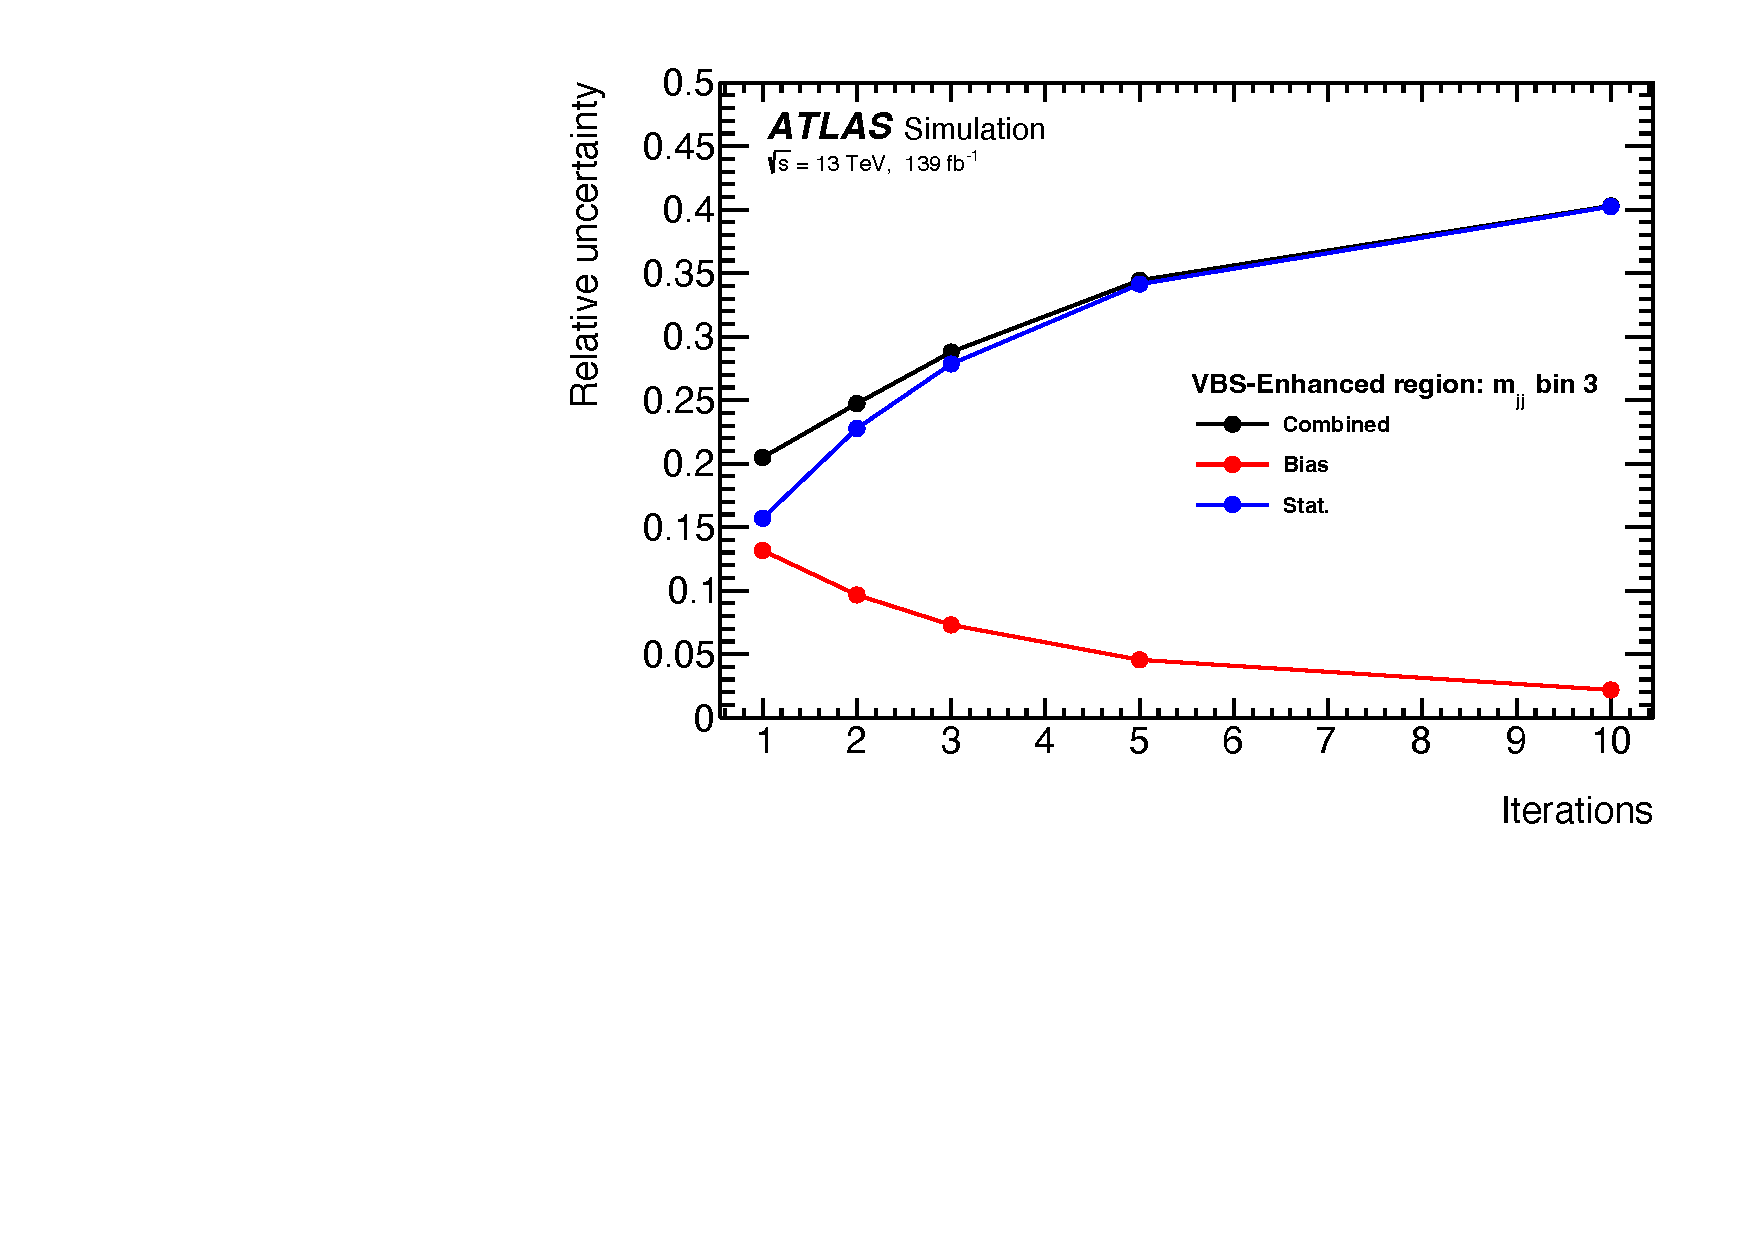
\includegraphics[width=.9\linewidth]{figures/Analysis/Unfolding/unfoldingbias/unfolding_bias_stat_unc_mjj_VBSEnh_bin3.pdf}
        \caption{ bin 3 }
    \end{subfigure}
    \begin{subfigure}{.48\textwidth}
        \centering
        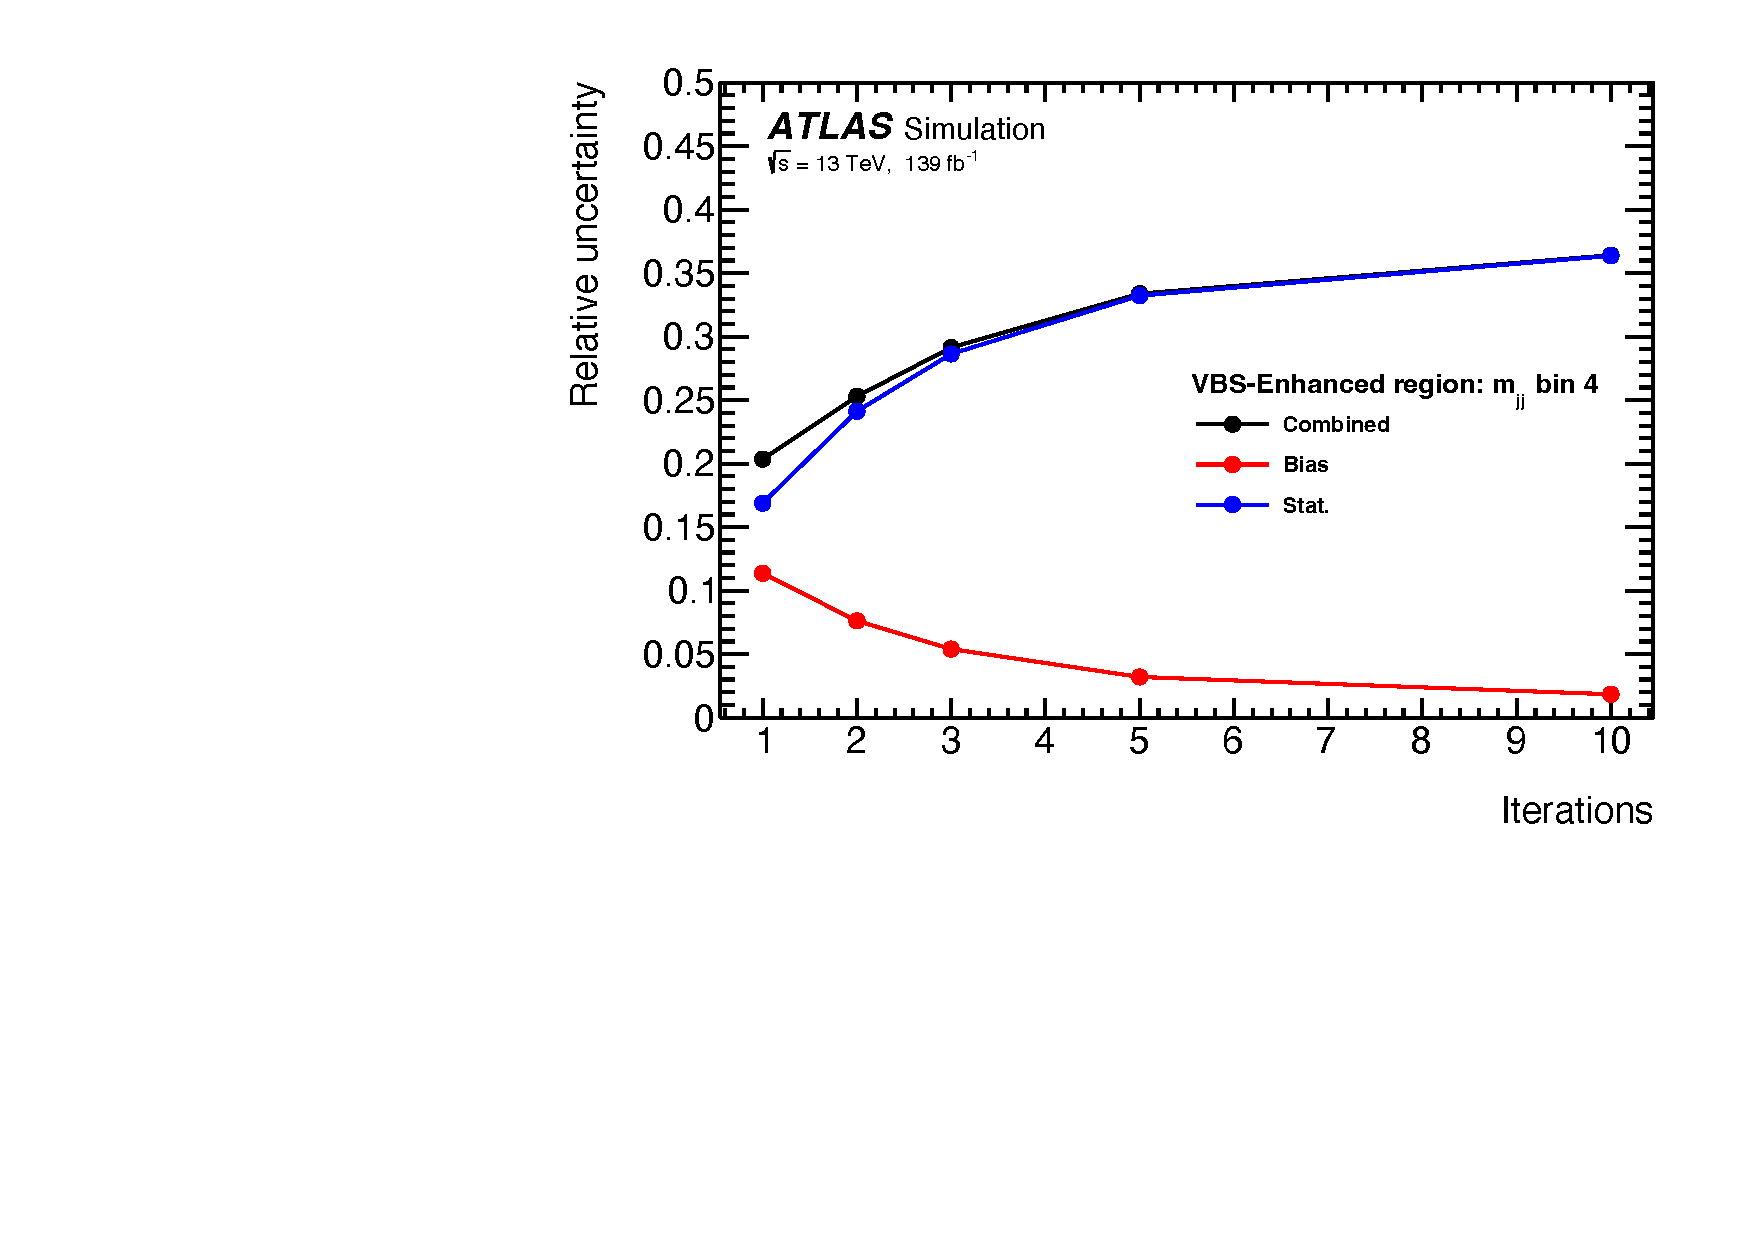
\includegraphics[width=.9\linewidth]{figures/Analysis/Unfolding/unfoldingbias/unfolding_bias_stat_unc_mjj_VBSEnh_bin4.pdf}
        \caption{bin 4 }
    \end{subfigure}
    \begin{subfigure}{.48\textwidth}
        \centering
        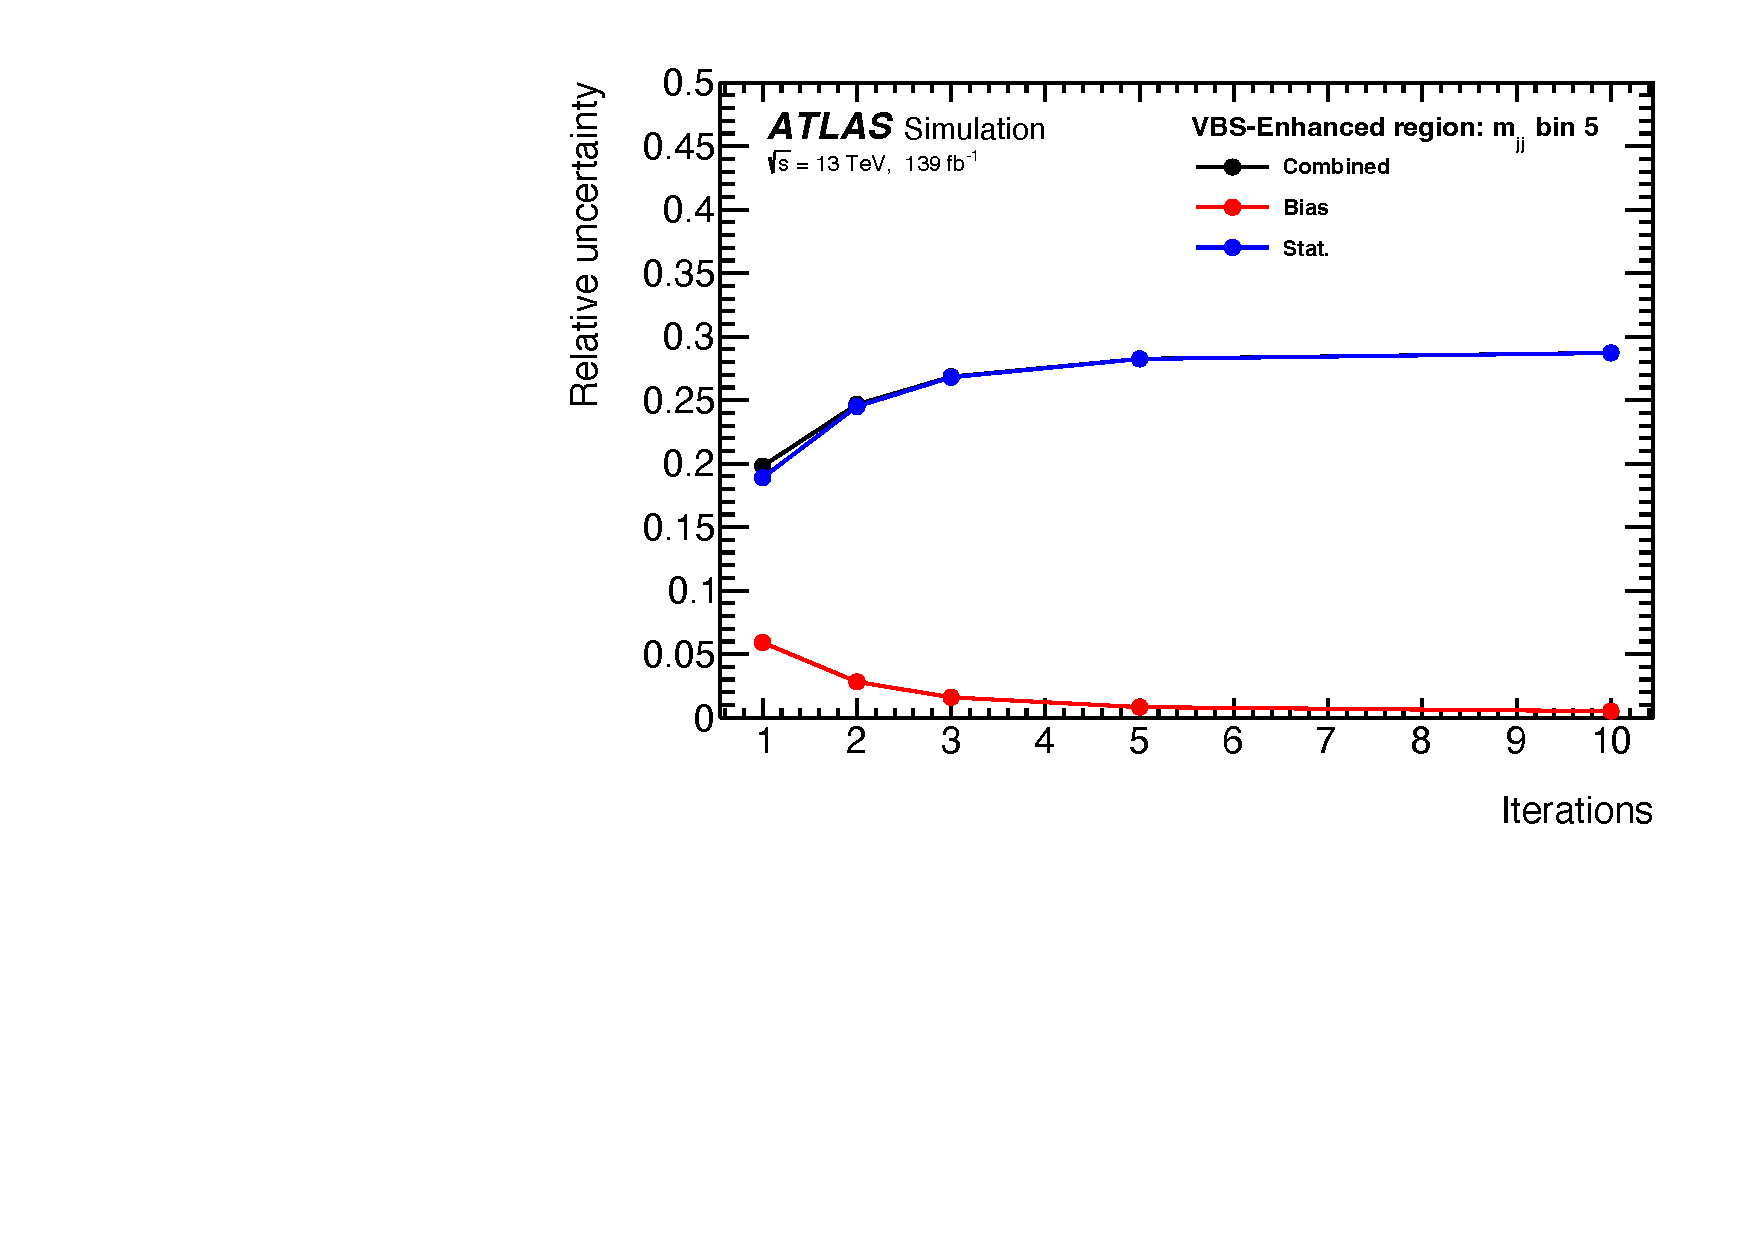
\includegraphics[width=.9\linewidth]{figures/Analysis/Unfolding/unfoldingbias/unfolding_bias_stat_unc_mjj_VBSEnh_bin5.pdf}
        \caption{bin 5 }
    \end{subfigure}
    \caption{ MC-toy-based unfolding bias and statistical uncertainty as a function of several numbers of iterations in each bin of $m_{jj}$ distribution in the VBS-Enhanced region. \label{fig:UnfoldingBiasStat_mjj_VBSEnhanced}}
\end{figure}

The unfolding bias is expected to converge to a value of zero with a higher number of iterations. However, as observed in figure \ref{fig:UnfoldingBiasStat_mjj_VBSEnhanced}, the rate of convergence of unfolding bias is lower, suggesting that the fiducial fakes present in the detector level distributions are not fully corrected by the unfolding method. The fiducial fraction, as shown by figure \ref{fig:UnfoldingInputs}, is usually between $60-80\%$ in this measurement. To confirm that a high fraction of fiducial fakes causes the unfolding bias, these are subtracted manually from the MC predictions of nominal and toy distributions. The MC-toy-based unfolding bias estimate is repeated and figure \ref{fig:UnfoldingBias_mjj_VBSEnhanced_noFakes} shows the resulting unfolding bias in each bin of $m_{jj}$ in the VBS-Enhanced region. Compared to the nominal unfolding bias shown in figure \ref{fig:UnfoldingBias_mjj_VBSEnhanced}, figure \ref{fig:UnfoldingBias_mjj_VBSEnhanced_noFakes} has a smaller bias in each bin. Moreover, the bias converges to zero at a higher rate.

\begin{figure}[htb]
    \centering
    \begin{subfigure}{.48\textwidth}
        \centering
        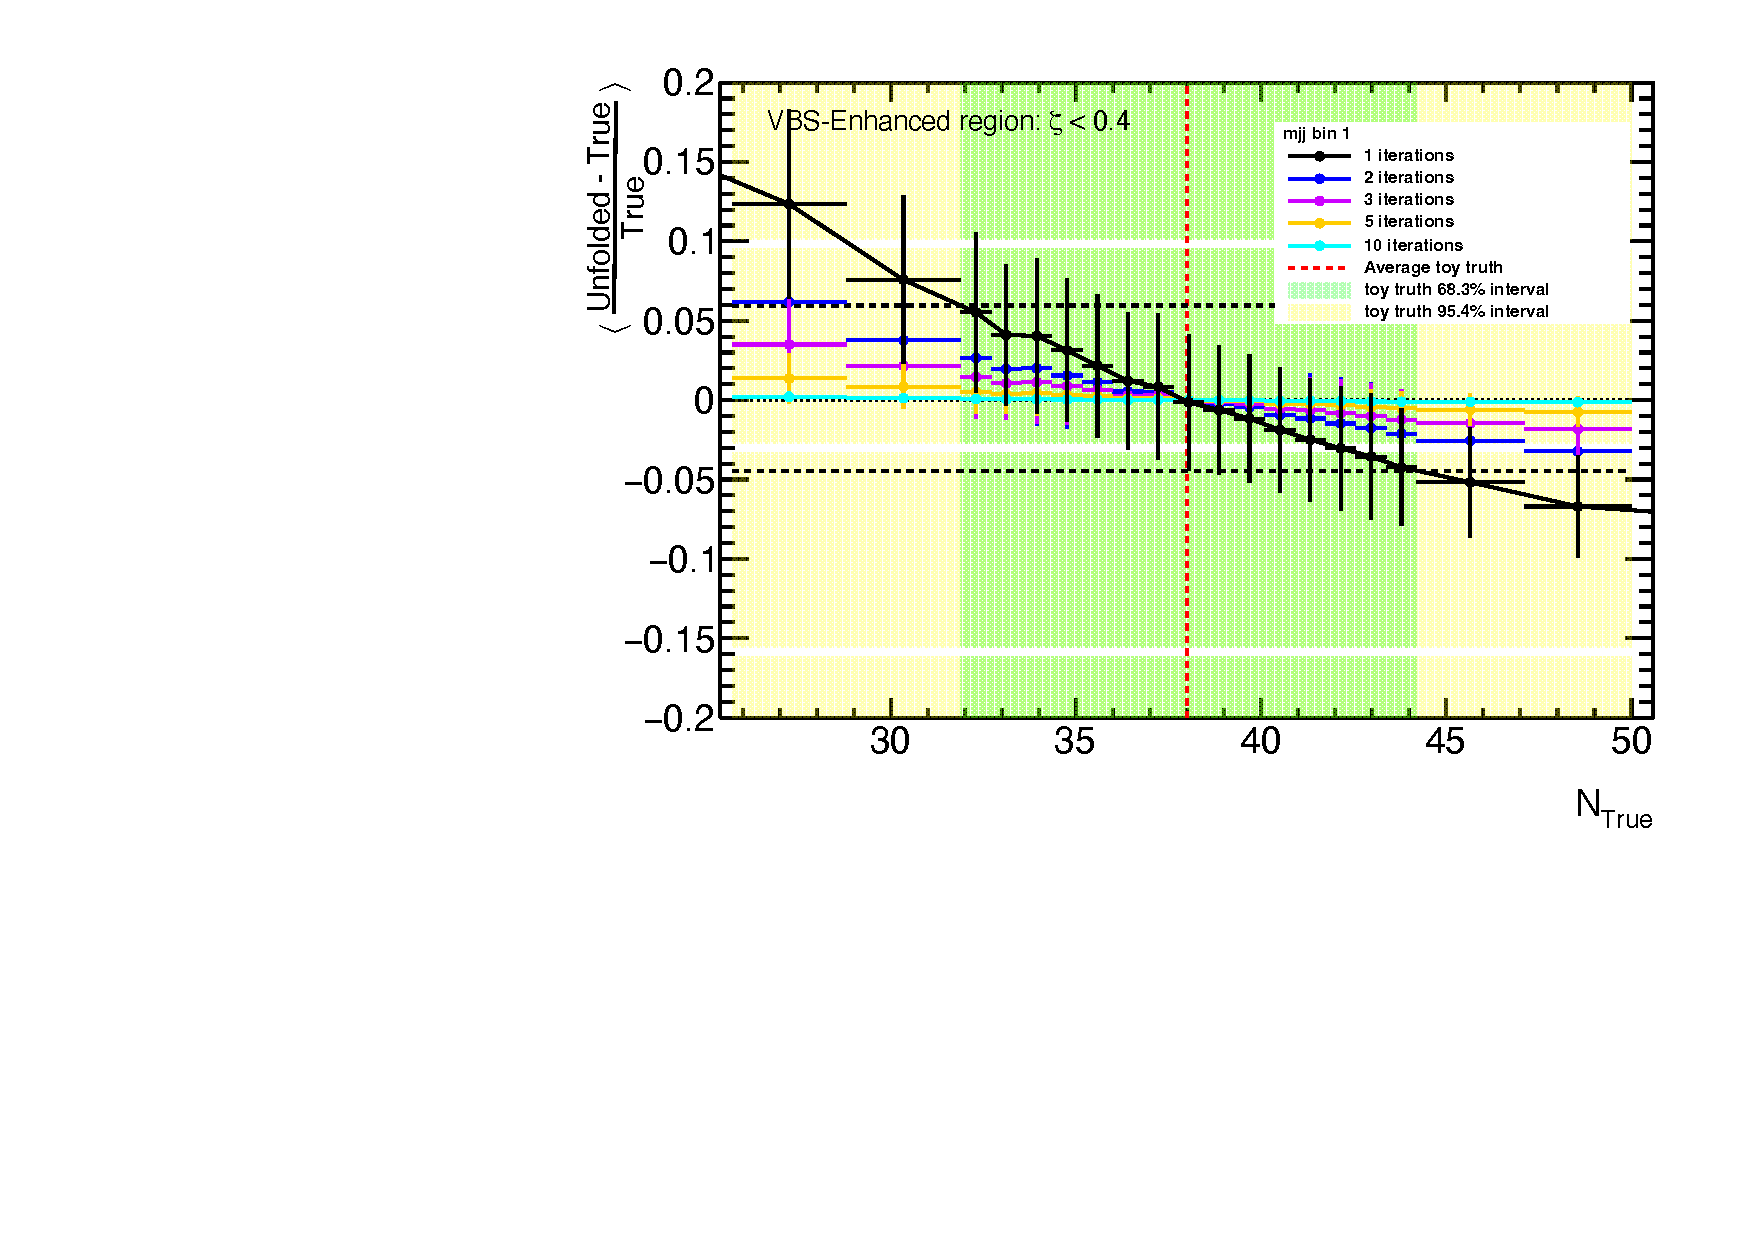
\includegraphics[width=.9\linewidth]{figures/Analysis/Unfolding/unfoldingbias/unfolding_bias_mjj_noFakes_VBSEnh_bin1.pdf}
        \caption{ bin 1}
    \end{subfigure}
    \begin{subfigure}{.48\textwidth}
        \centering
        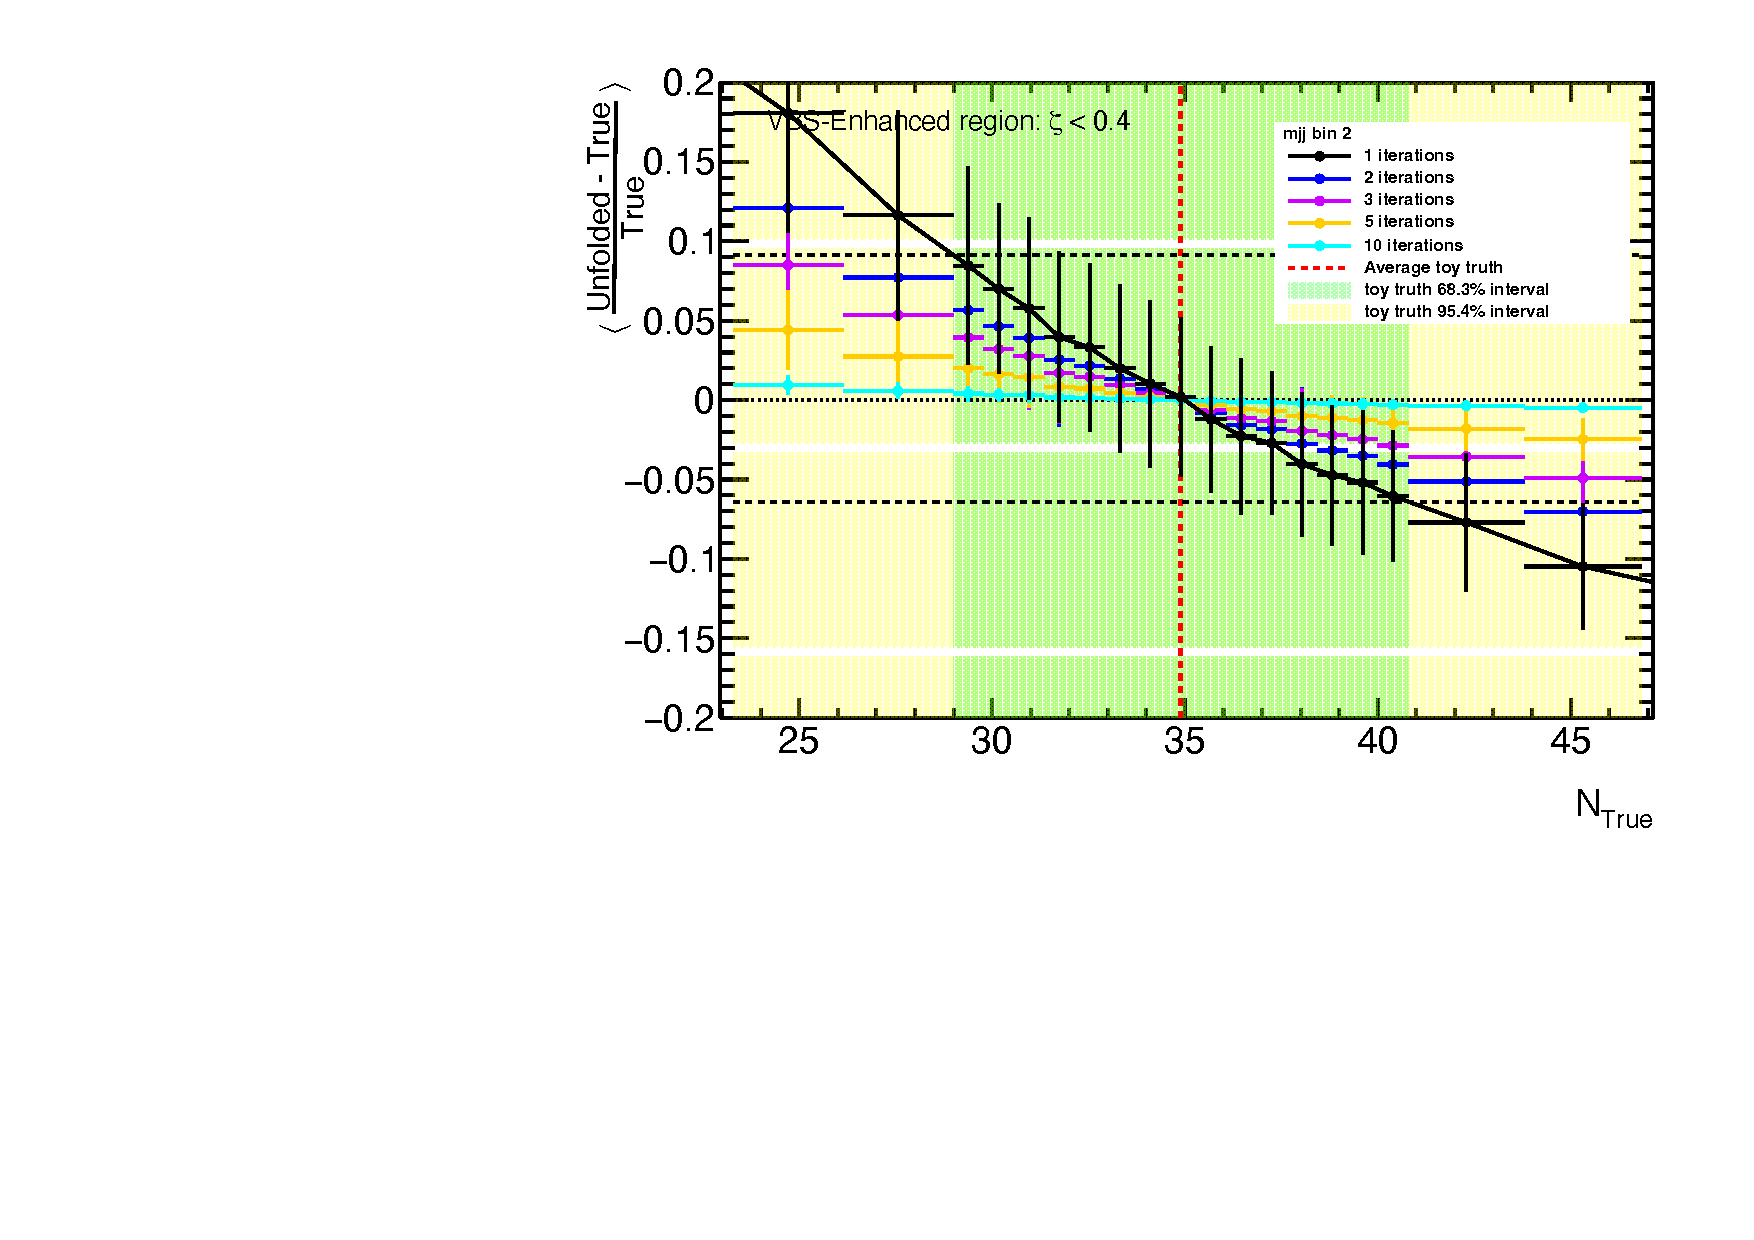
\includegraphics[width=.9\linewidth]{figures/Analysis/Unfolding/unfoldingbias/unfolding_bias_mjj_noFakes_VBSEnh_bin2.pdf}
        \caption{bin 2 }
    \end{subfigure}\\
    \begin{subfigure}{.48\textwidth}
        \centering
        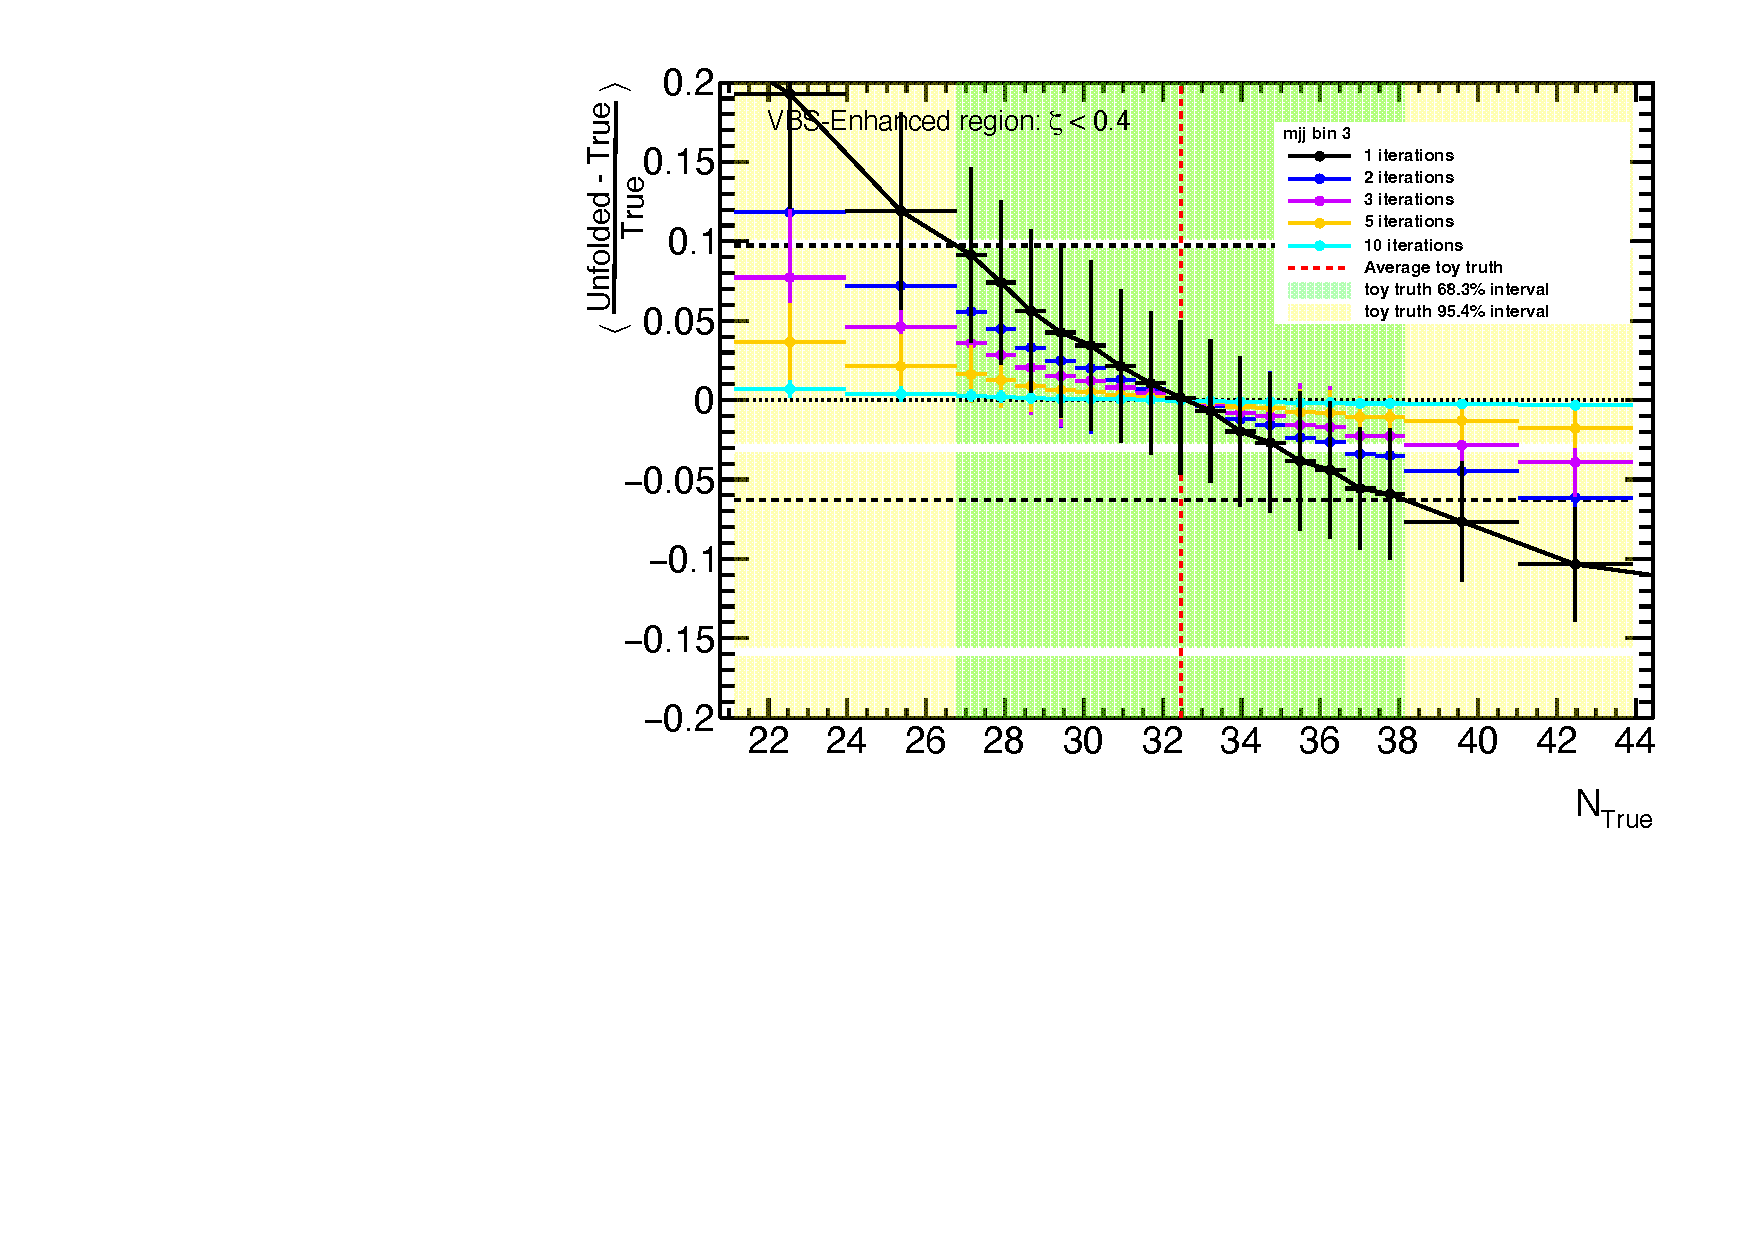
\includegraphics[width=.9\linewidth]{figures/Analysis/Unfolding/unfoldingbias/unfolding_bias_mjj_noFakes_VBSEnh_bin3.pdf}
        \caption{ bin 3 }
    \end{subfigure}
    \begin{subfigure}{.48\textwidth}
        \centering
        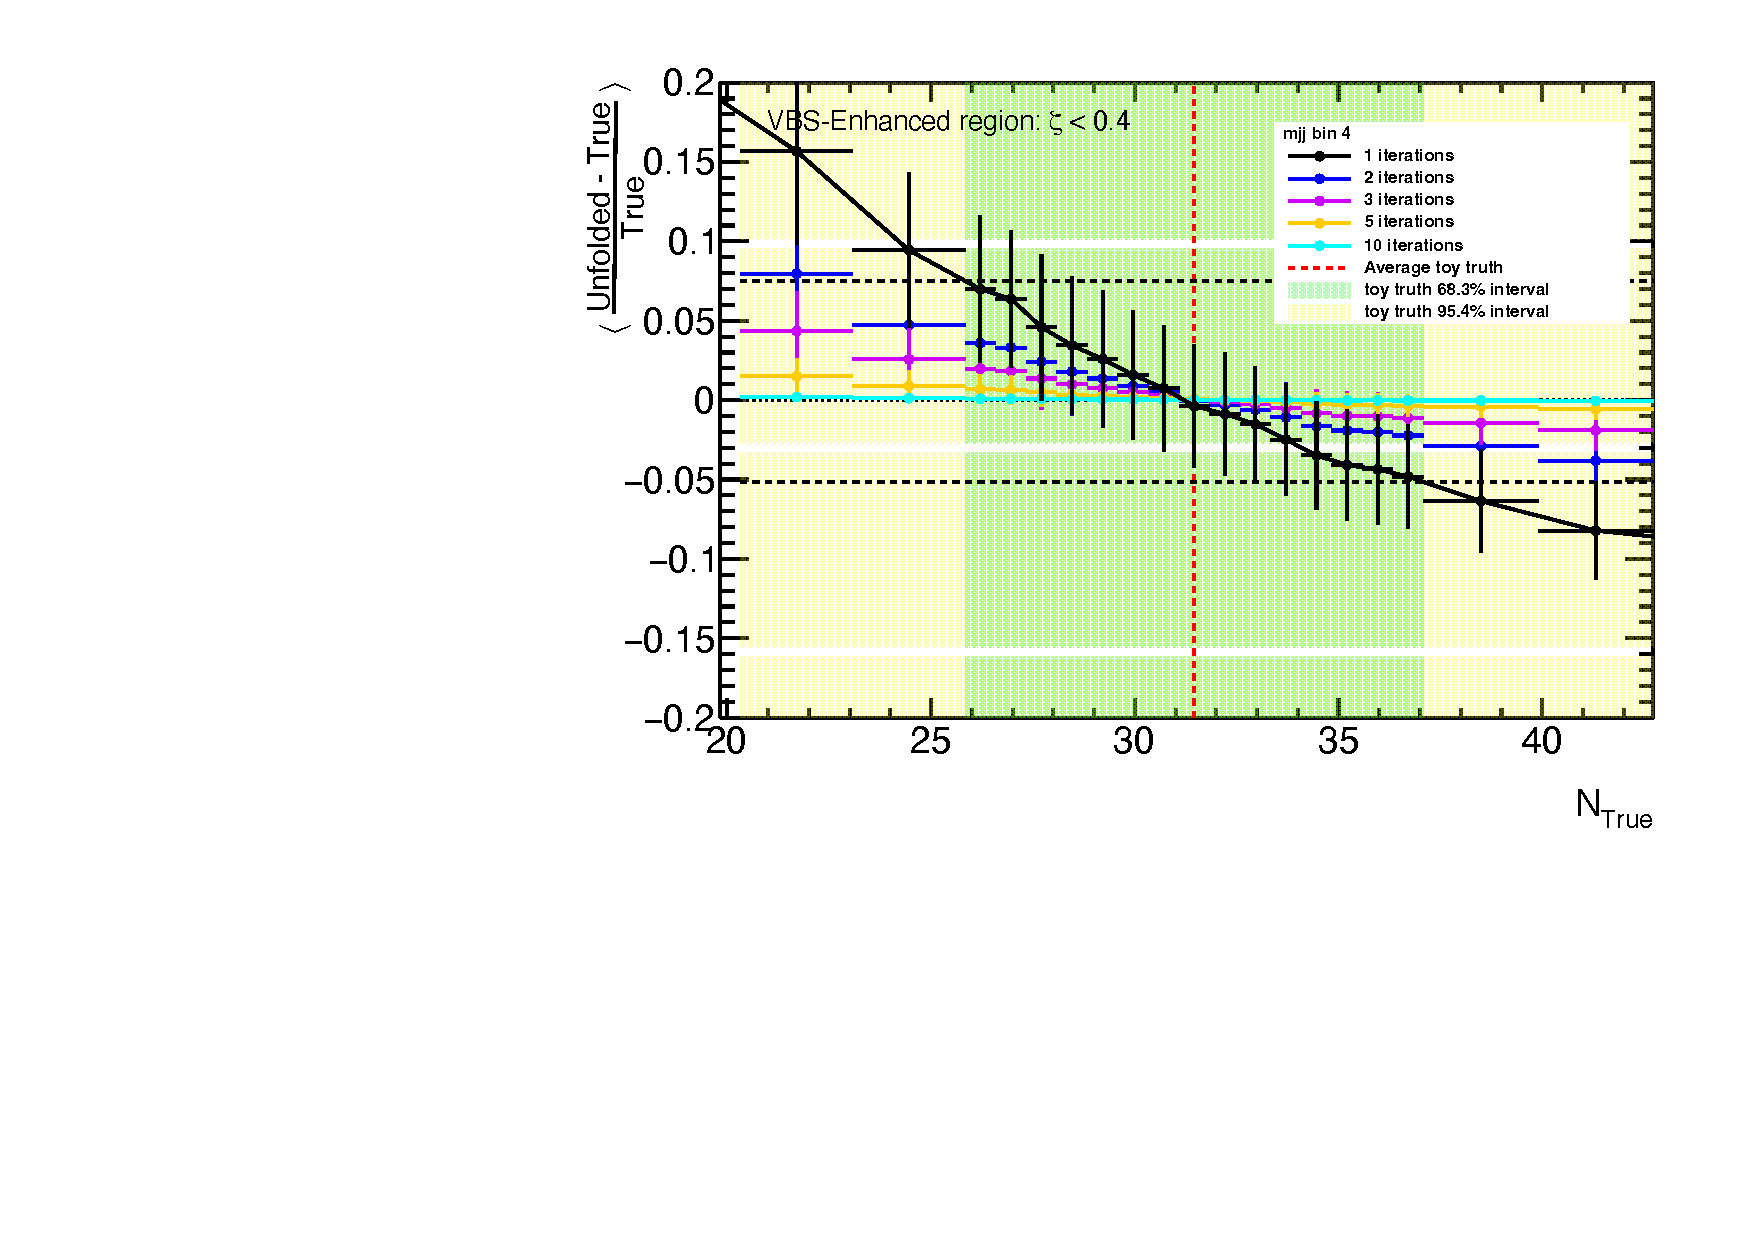
\includegraphics[width=.9\linewidth]{figures/Analysis/Unfolding/unfoldingbias/unfolding_bias_mjj_noFakes_VBSEnh_bin4.pdf}
        \caption{bin 4 }
    \end{subfigure}
    \begin{subfigure}{.48\textwidth}
        \centering
        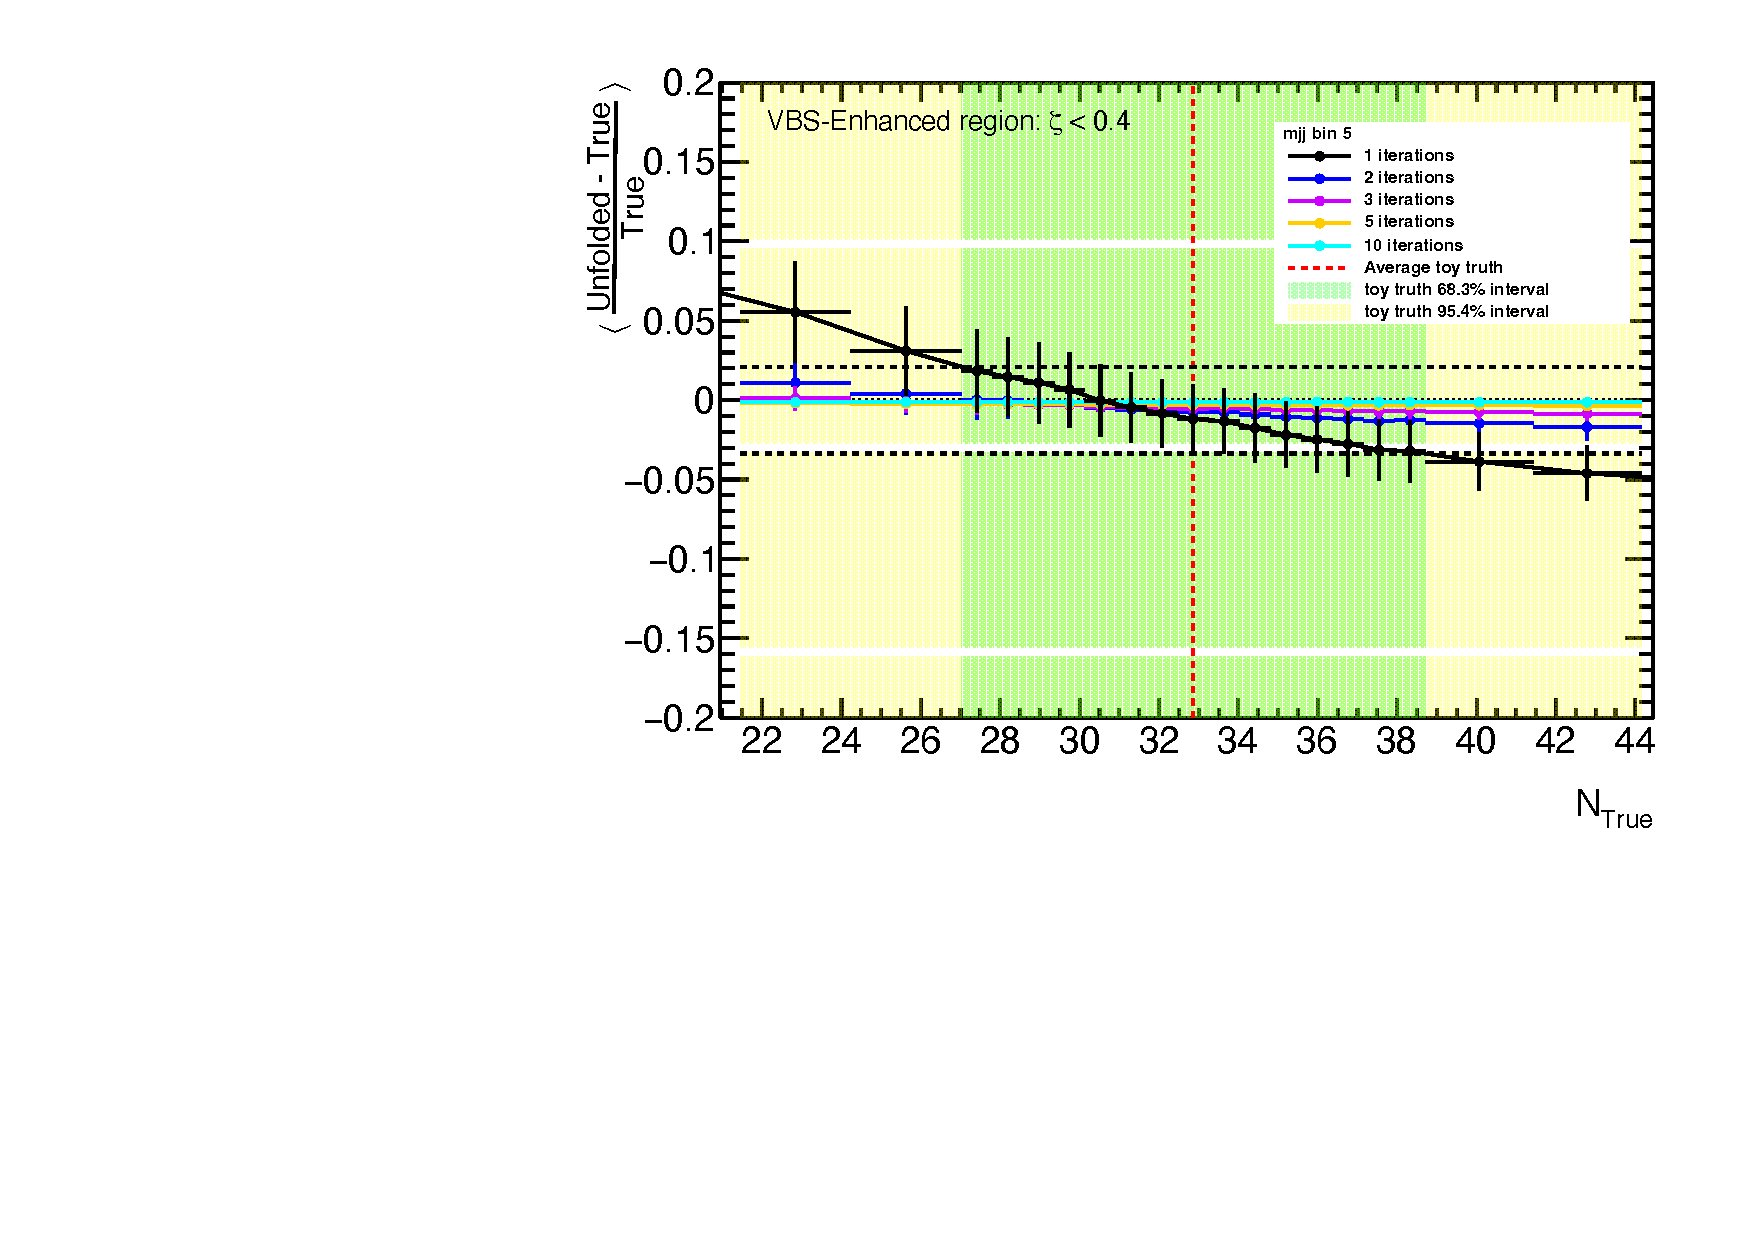
\includegraphics[width=.9\linewidth]{figures/Analysis/Unfolding/unfoldingbias/unfolding_bias_mjj_noFakes_VBSEnh_bin5.pdf}
        \caption{bin 5 }
    \end{subfigure}
    \caption{ MC-toy-based unfolding bias in each bin of $m_{jj}$ in the VBS-Enhanced region using Gaussian toys after subtracting the contribution of the fiducial fake events from both nominal and toy MC predictions.\label{fig:UnfoldingBias_mjj_VBSEnhanced_noFakes}}
\end{figure}

The differential measurements of the $ZZ(\rightarrow 4\ell)jj$ process are statistically limited, so it is impossible to directly subtract the fiducial fakes from data without increasing both statistical and systematic uncertainties from the fiducial fake estimate. However, it is imperative to understand the origin and topology of the fiducial fake events to reduce their impact without degrading the unfolding procedure's performance. Figure \ref{fig:fake_fraction_jets} shows the fake fraction, the fraction of detector-level events passing detector-level selection but failing the particle-level selection as a function of $p_{T}$ (left) and $\eta$ (right) of the leading and the sub-leading jets. More significant fractions of fakes are observed in low-$p_{T}$ and high $\eta$ region, which is likely related to the worse resolution of jet reconstruction in low-$p_{T}$ and smaller efficiency of fJVT tagging in forward regions. The large fraction of fiducial fakes is understood to originate either from migrations outside the fiducial volume due to jet resolution effects or from wrongfully selecting events with pile-up jets. More stringer kinematic selections were applied to the leading and sub-leading jets in an attempt to reduce the bias, but this resulted in the degradation of unfolding performance due to low statistics. Therefore, the nominal bias shown in Section \ref{subsec:UnfoldingUnc} was deemed optimal. 

\begin{figure}[htb]
    \centering
    \begin{subfigure}{.48\textwidth}
        \centering
        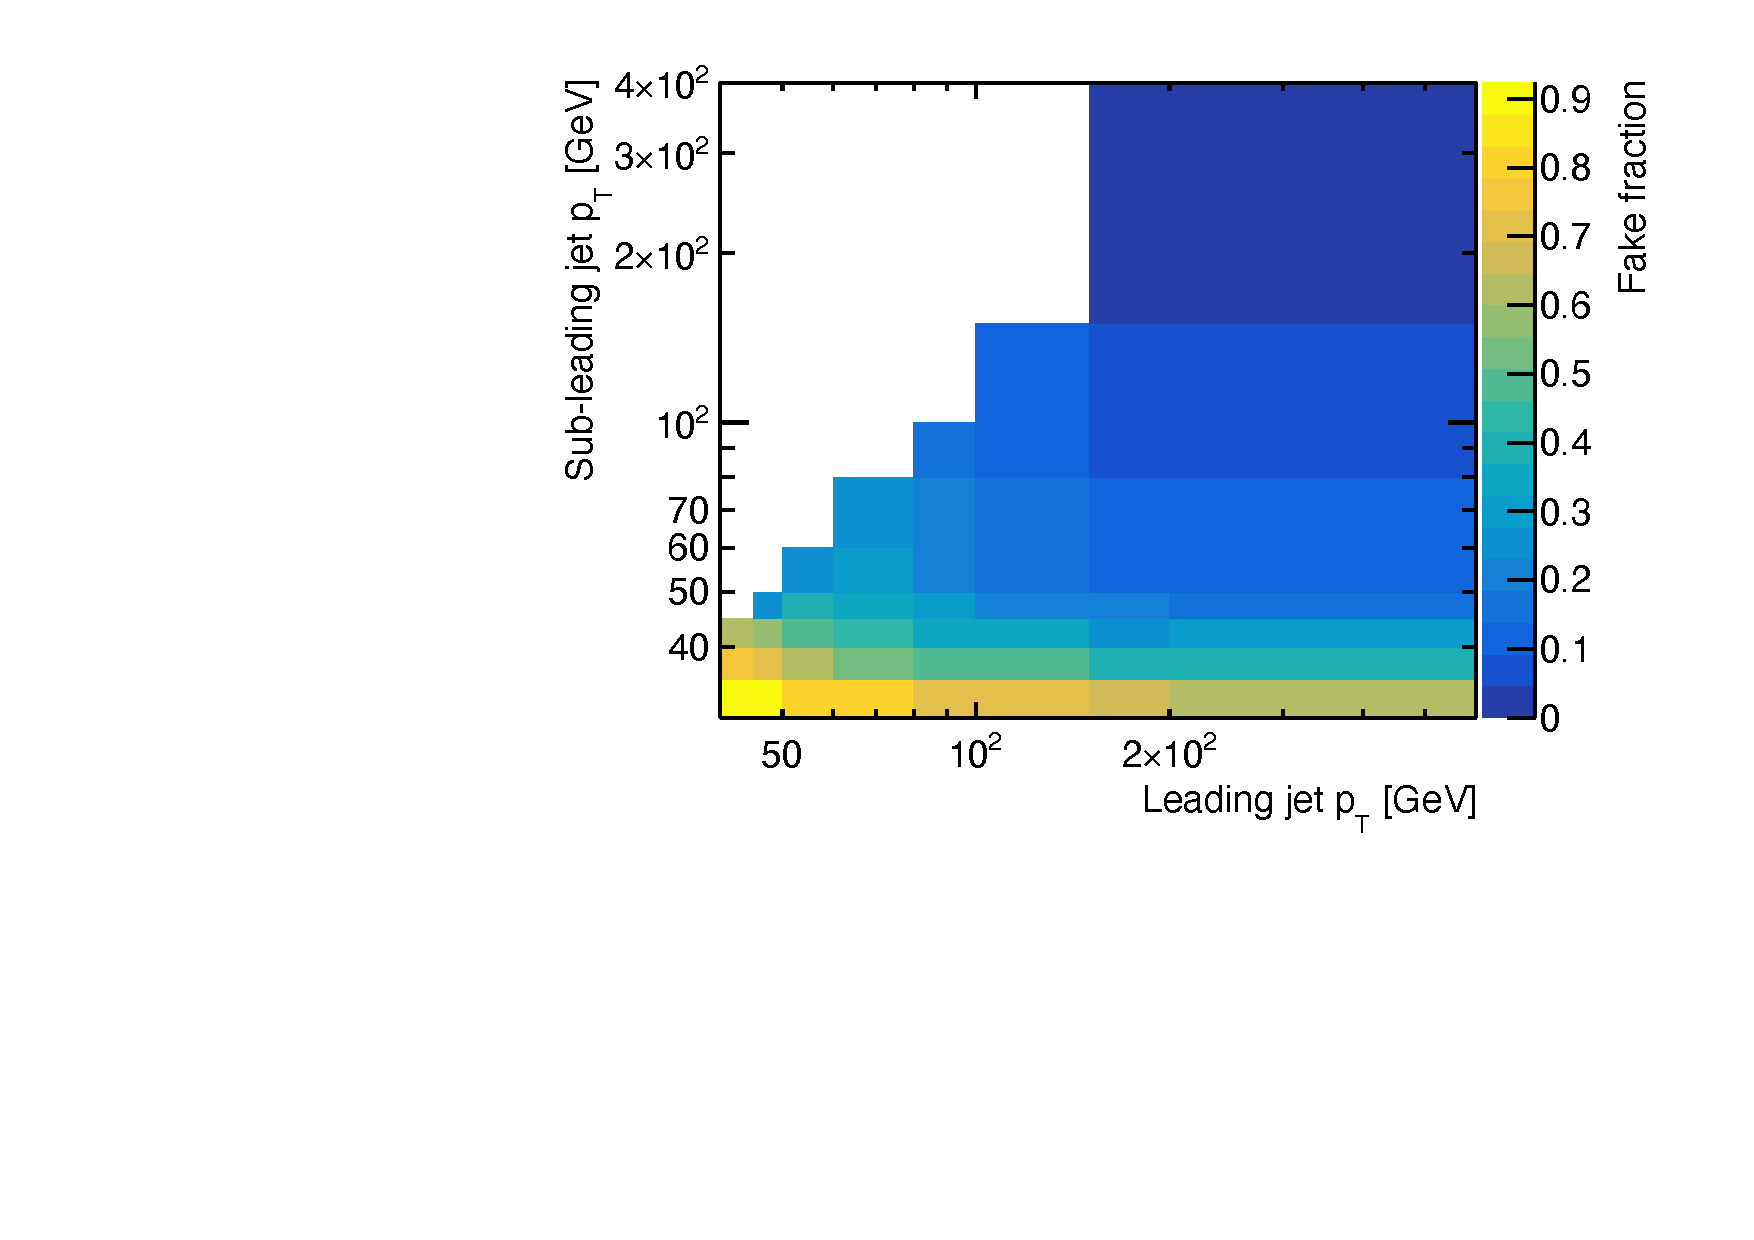
\includegraphics[width=.9\linewidth]{figures/Analysis/Unfolding/FakeFraction_pt_jets.pdf}
        \caption{ $p_{T}$}
    \end{subfigure}
    \begin{subfigure}{.48\textwidth}
        \centering
        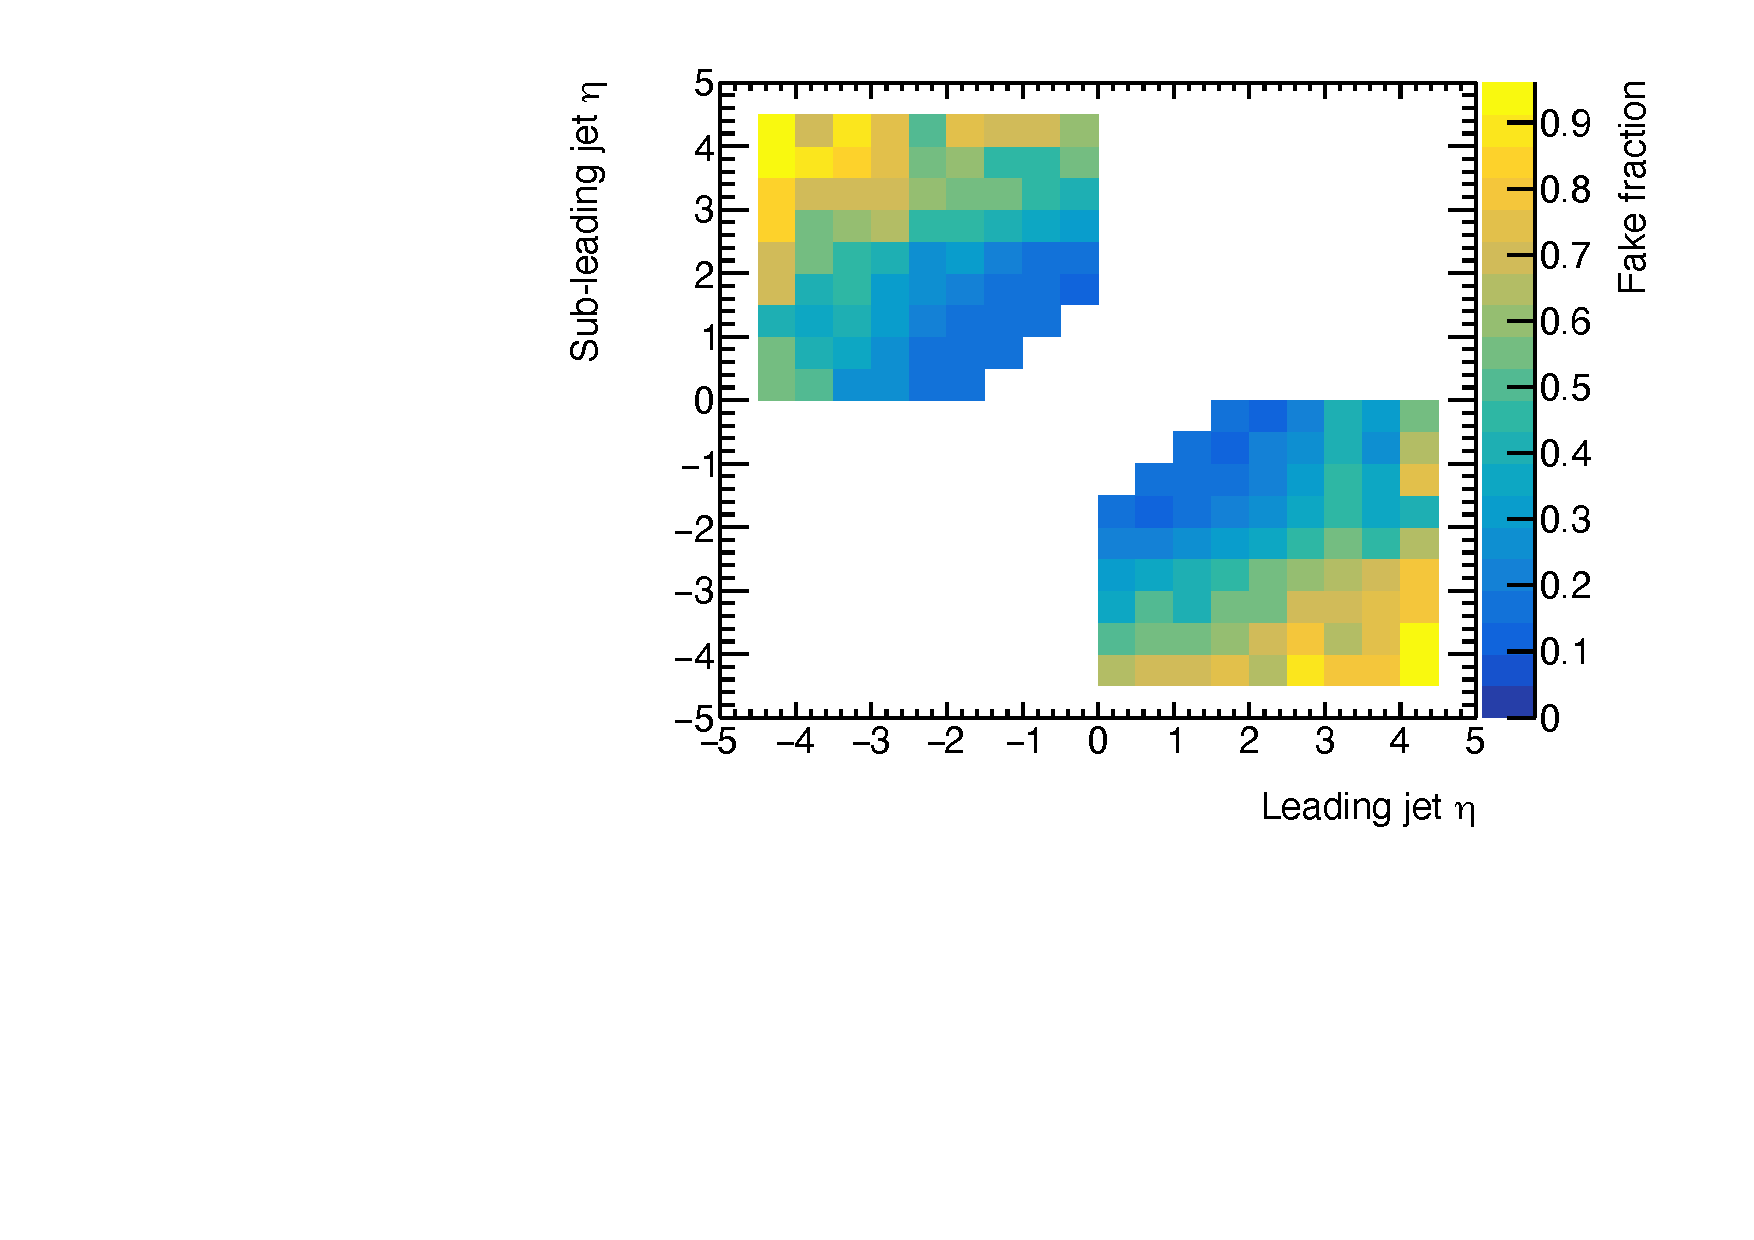
\includegraphics[width=.9\linewidth]{figures/Analysis/Unfolding/FakeFraction_eta_jets.pdf}
        \caption{$\eta$}
    \end{subfigure}
    \caption{ Fraction of fiducial fake events as a function of $p_{T}~\&~\eta$ of the leading and the sub-leading jets in the VBS-Enhanced region.\label{fig:fake_fraction_jets}}
\end{figure}

\section{VBS Suppressed Region}
\label{Appendix:VBSSupRegion}
This section summarizes the results of the detector level yield and the unfolded differential cross-sections measured in the VBS-Suppressed region. The systematics affecting these results are also discussed briefly.

\subsection{Systematics}
\label{appendix:VBSSupSys}
The same systematic uncertainties discussed in Chapter $V$ also impact the measurements in the VBS-Suppressed region. Table \ref{tab:systematics_mjj_VBS_Suppressed} shows the impact of several systematic uncertainties on the unfolded differential cross-sections in each bin of $m_{jj}$ for the VBS-Suppressed region. Like the VBS-Enhanced region, unfolding bias followed by the jet-related uncertainties and QCD MC modeling uncertainty are the most significant sources of systematic uncertainties. Figure \ref{fig:sys_mjj_VBS_Suppressed_total} shows the impact of the statistical and different systematic uncertainties on the unfolded cross-sections as a function of $m_{jj}$. The unfolded cross-sections are statistically limited. Figure \ref{fig:sys_mjj_VBS_Suppressed_jet} shows the breakdown of the jet-related uncertainties, where uncertainties related to the punch through calibration are the dominant source.  

\begin{table}
    \centering
    \caption{Breakdown of the relative systematic uncertainties ($\%$) for each bin of $\mjj$ in the VBS-Suppressed region. \label{tab:systematics_mjj_VBS_Suppressed}}
    \begin{tabular}{|l || c | c | c | }
    \hline 
    Bin $m_{jj}$ [GeV] & [300, 410) & [410, 600) & [600, 1780)\\
    \hline 
    QCD MC modelling & 2 & 0.16 & \textbf{7.1}\\
    Jet & \textbf{7.3} & \textbf{6.8} & \textbf{6.2 }\\
    Trigger & 0.03 & 0.06 & 0.08 \\
    Leptons & 1.4 & 1.5 & 1.6 \\
    PRW & 0.39 & 0.06 & 0.16\\
    Theory ($qqZZ$) & 1.9 & 2.3 & 2.1 \\
    Theory (EWK $qqZZjj$) & 0.02 & 0.02 & 0.04 \\
    Theory ($ggZZ$) & 0.13 & 0.22 & 0.28 \\
    MC Bkg. (ttV+VVV) & 1.6 & 1.7 & 1.6 \\
    Fake Bkg. (stat + syst) & 3.4 & 2.9 & 2.6 \\
    Luminosity & 1.5 & 1.4 & 1.4 \\
    Unfolding Bias & \textbf{12.1} & \textbf{11.0} & \textbf{6.1}\\
    \hline
    Total & 14.7 & 13.6 & 12.0 \\
    \hline
    \end{tabular}
\end{table}

\begin{figure}[!htb]
    \centering
    \begin{subfigure}{.48\textwidth}
        \centering
        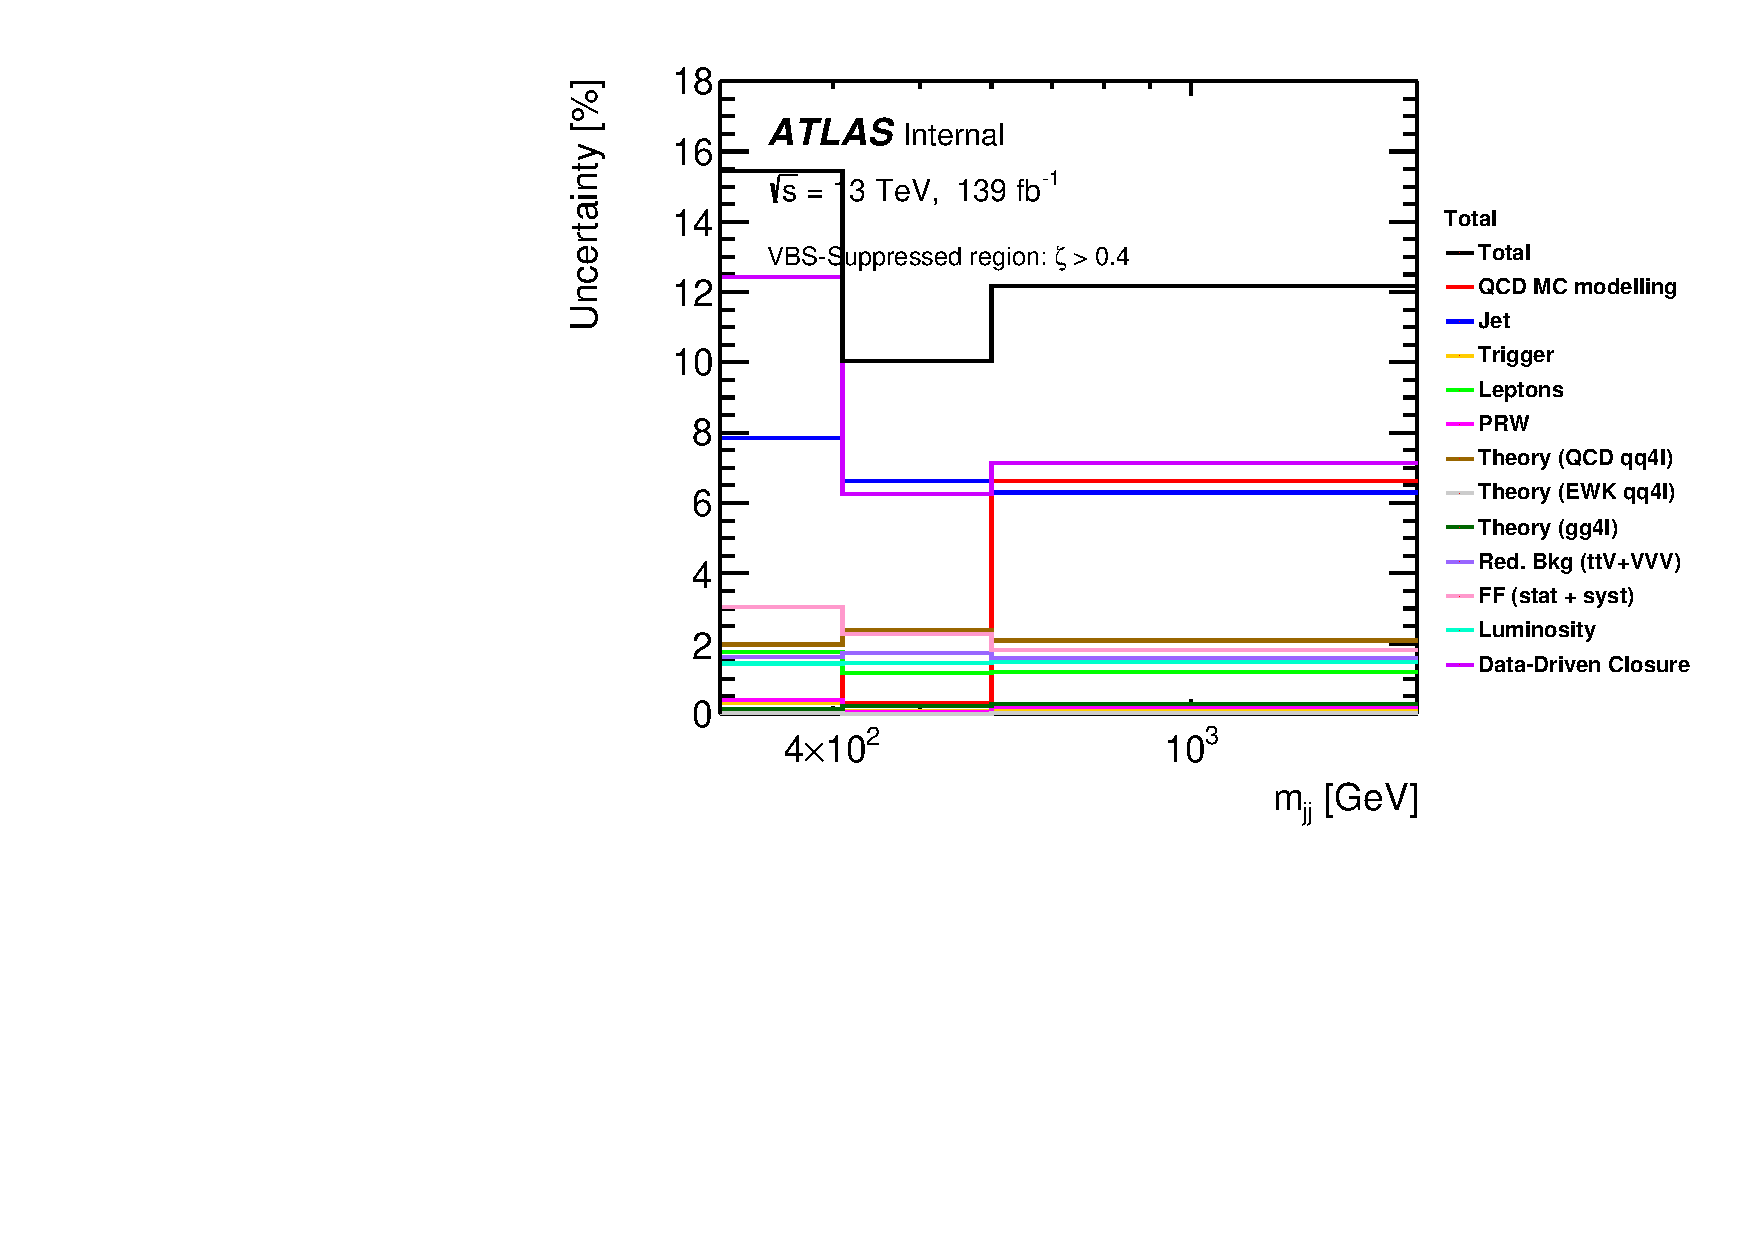
\includegraphics[width=.9\linewidth]{figures/Analysis/Systematics/systematics_VBS_Suppressed.pdf}
        \caption{ Statistical and systematic uncertainties are affecting the differential cross-section measurements. \label{fig:sys_mjj_VBS_Suppressed_total}}
    \end{subfigure}
    \begin{subfigure}{.48\textwidth}
        \centering
        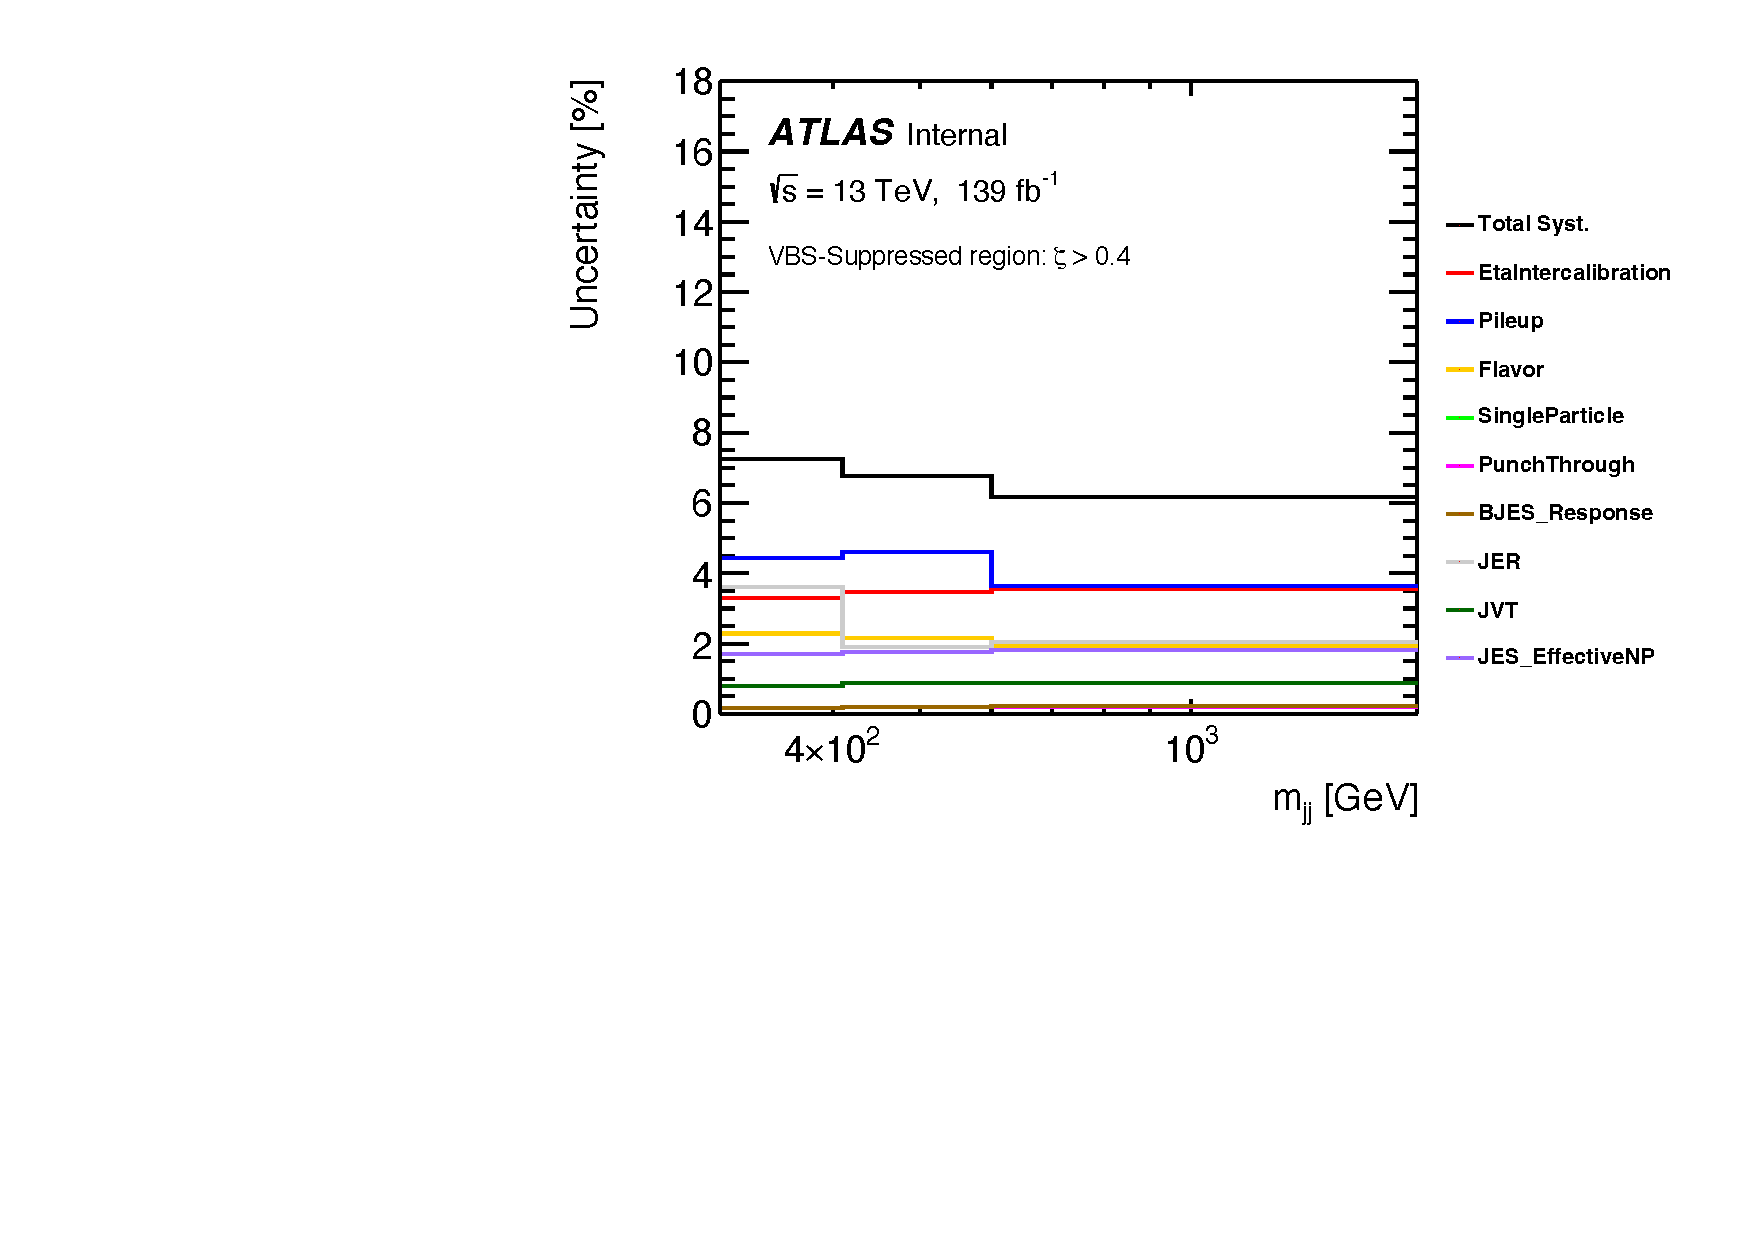
\includegraphics[width=.9\linewidth]{figures/Analysis/Systematics/jet_systematics_VBS_Suppressed.pdf}
        \caption{Breakdown of the total jet-related uncertainties. \label{fig:sys_mjj_VBS_Suppressed_jet} }
    \end{subfigure}
    \caption{Uncertainties as a function of $\mjj$ in the VBS-Suppressed region.}  \label{fig:sys_mjj_VBS_Suppressed}
\end{figure}

\subsection{Detector Level Measurements}
\label{appendix:VBSSupReco}

Figures \ref{fig:reco_VBS_Suppressed_a} and \ref{fig:reco_VBS_Suppressed_b} show the measured data yield compared to the SM detector-level predictions as a function of the eleven kinematic observables in the VBS-Suppressed region. Distributions are statistically limited, and the impact of theoretical and experimental systematic uncertainties ranges from about $20$ to $30\%$ depending on bins and distributions. Similar to the VBS-Enhanced region, a $\chi^2/NDF$ for each distribution is also reported. These values suggest a good agreement between the measured data and the SM prediction. 

\begin{figure}[!htb]
    \centering
    \begin{subfigure}{.49\textwidth}
        \centering
        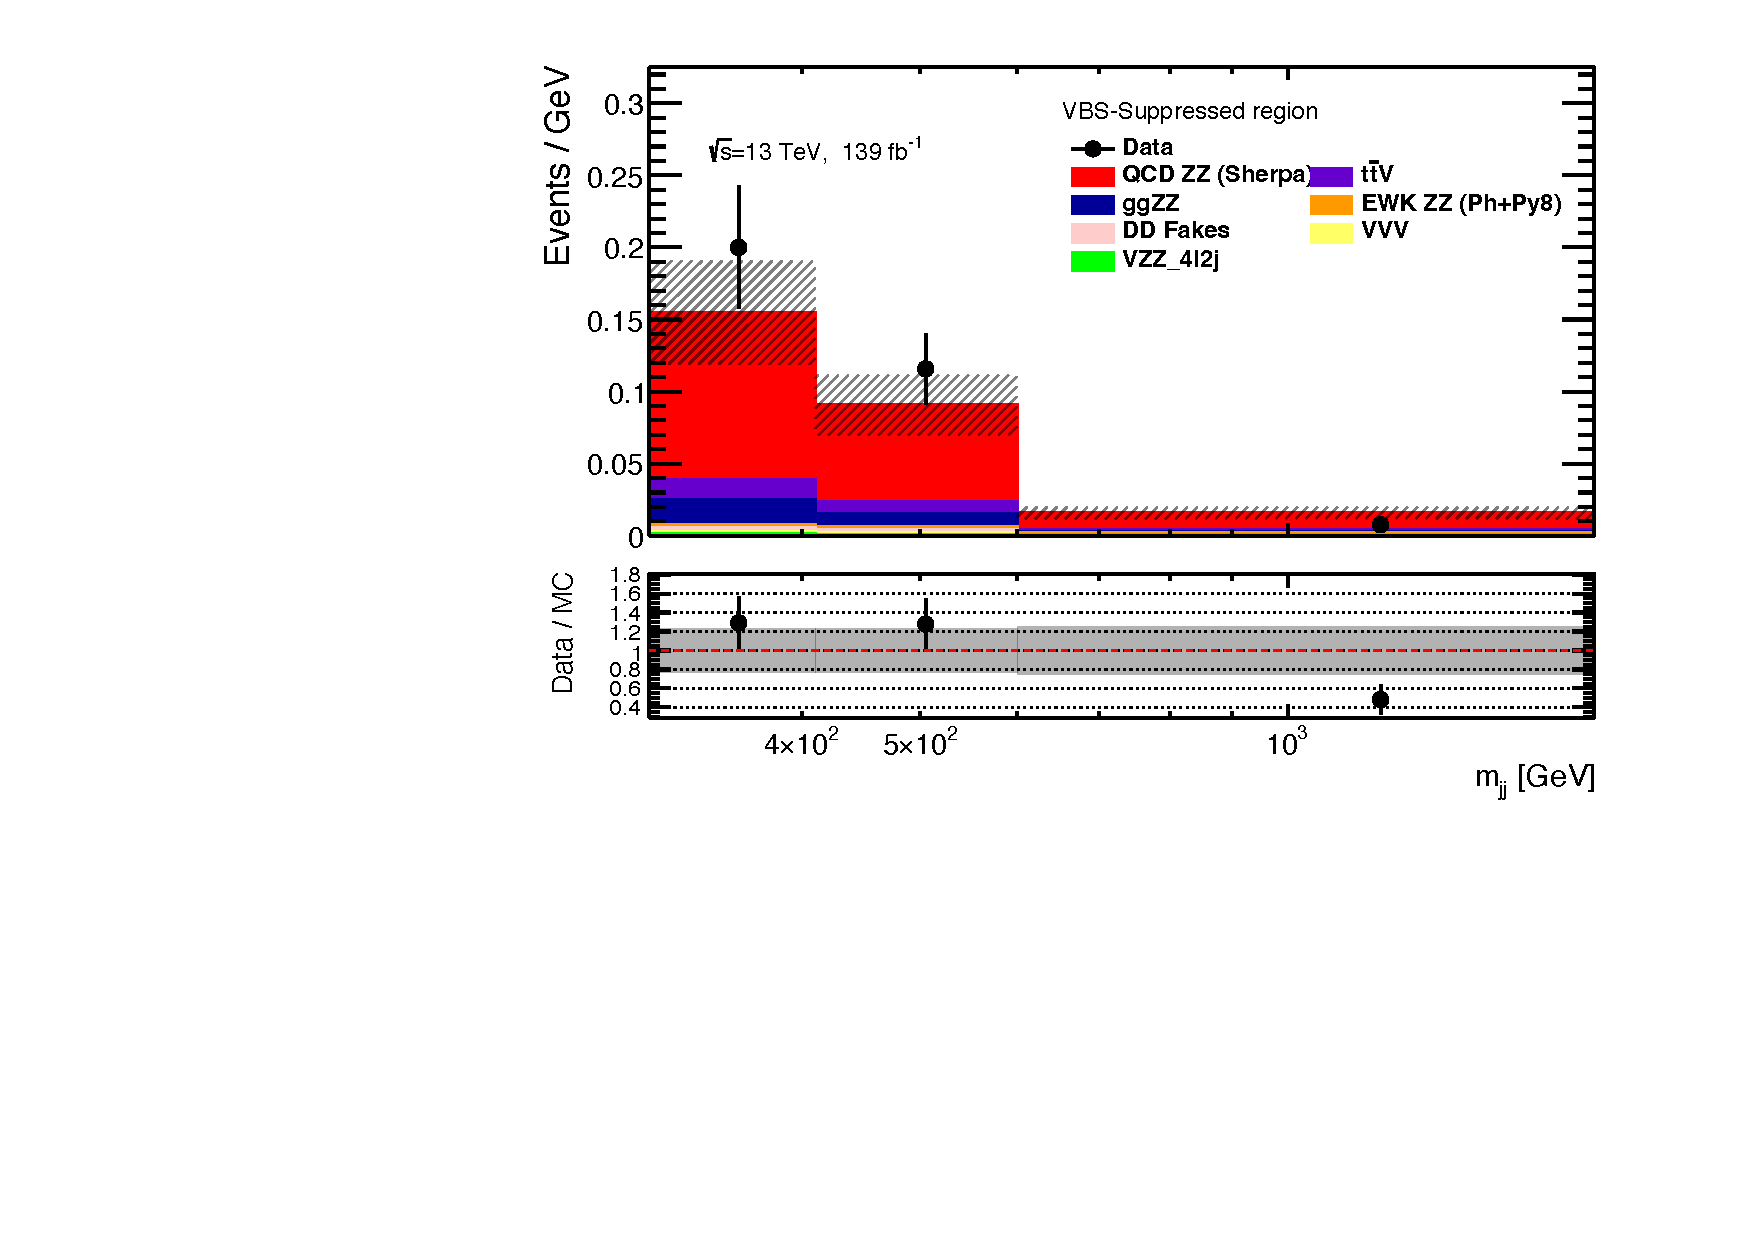
\includegraphics[width=.98\linewidth]{figures/Results/RecoDist_VBSSuppressed/reco_mjj_CR.pdf}
        \caption{ \footnotesize{$m_{jj}$}: $\chi^2/NDF = 1.78$ }
    \end{subfigure}
    \begin{subfigure}{.49\textwidth}
        \centering
        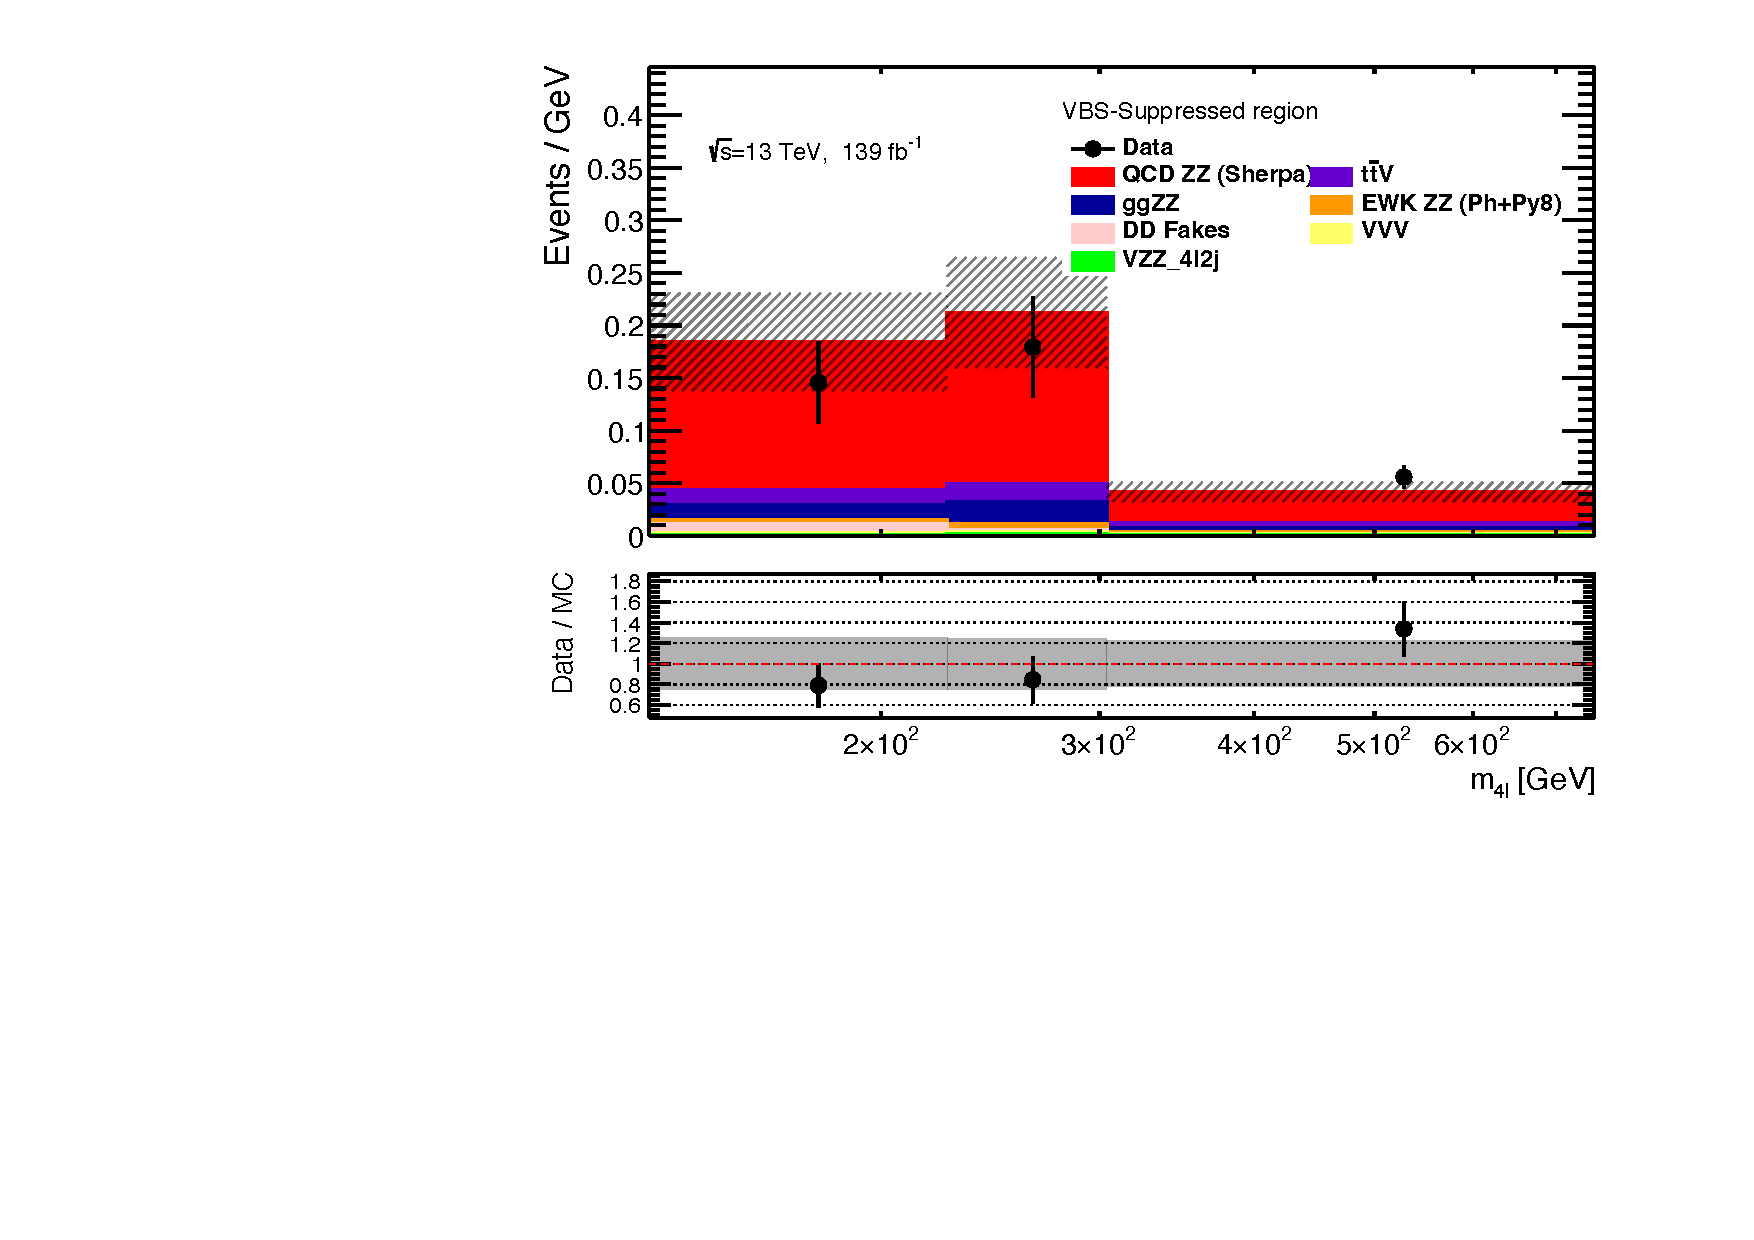
\includegraphics[width=.98\linewidth]{figures/Results/RecoDist_VBSSuppressed/reco_m4l_CR.pdf}
        \caption{ \footnotesize{$m_{4\ell}$ }: $\chi^2/NDF = 0.88$ }
    \end{subfigure}\\
    \begin{subfigure}{.49\textwidth}
        \centering
        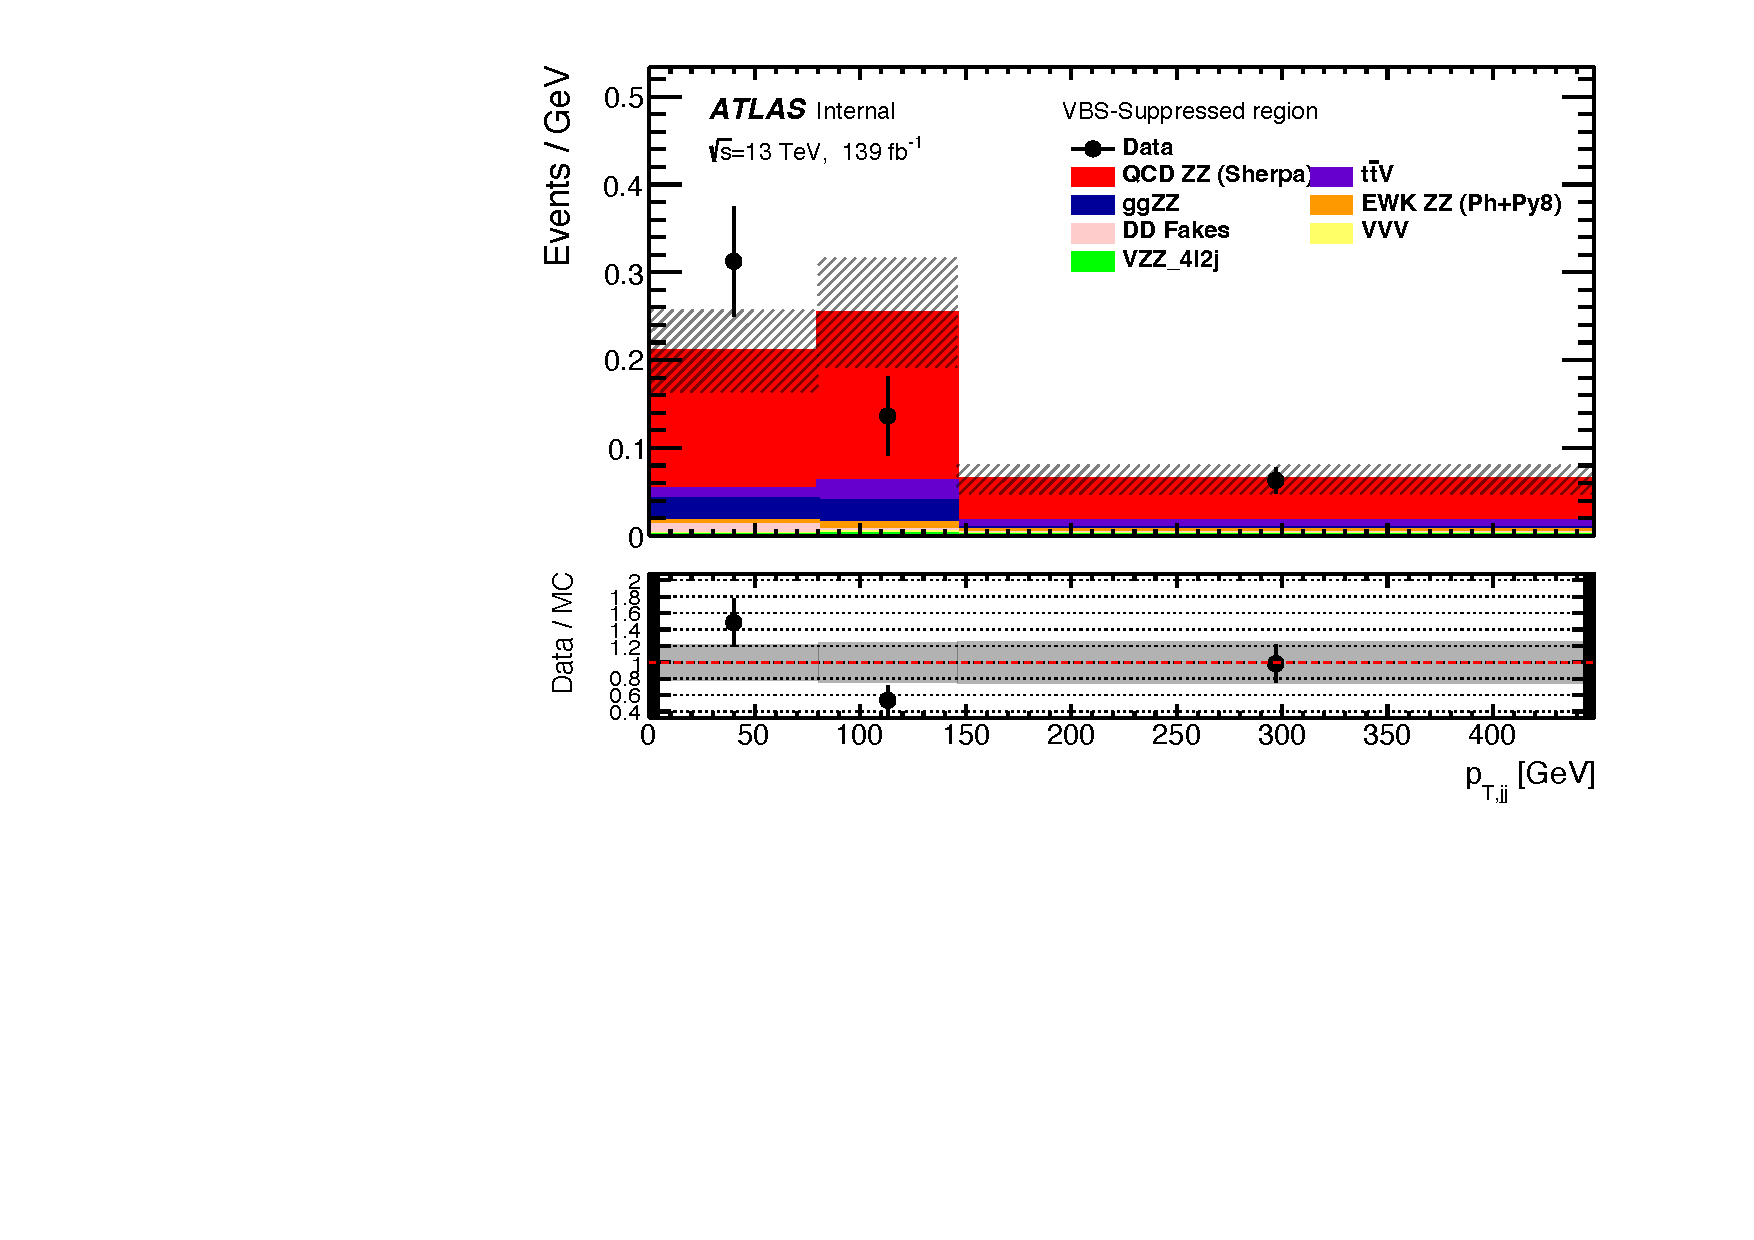
\includegraphics[width=.98\linewidth]{figures/Results/RecoDist_VBSSuppressed/reco_ptjj_CR.pdf}
        \caption{ \footnotesize{$p_{T,jj}$}: $\chi^2/NDF = 2.0$ }
    \end{subfigure}
    \begin{subfigure}{.49\textwidth}
        \centering
        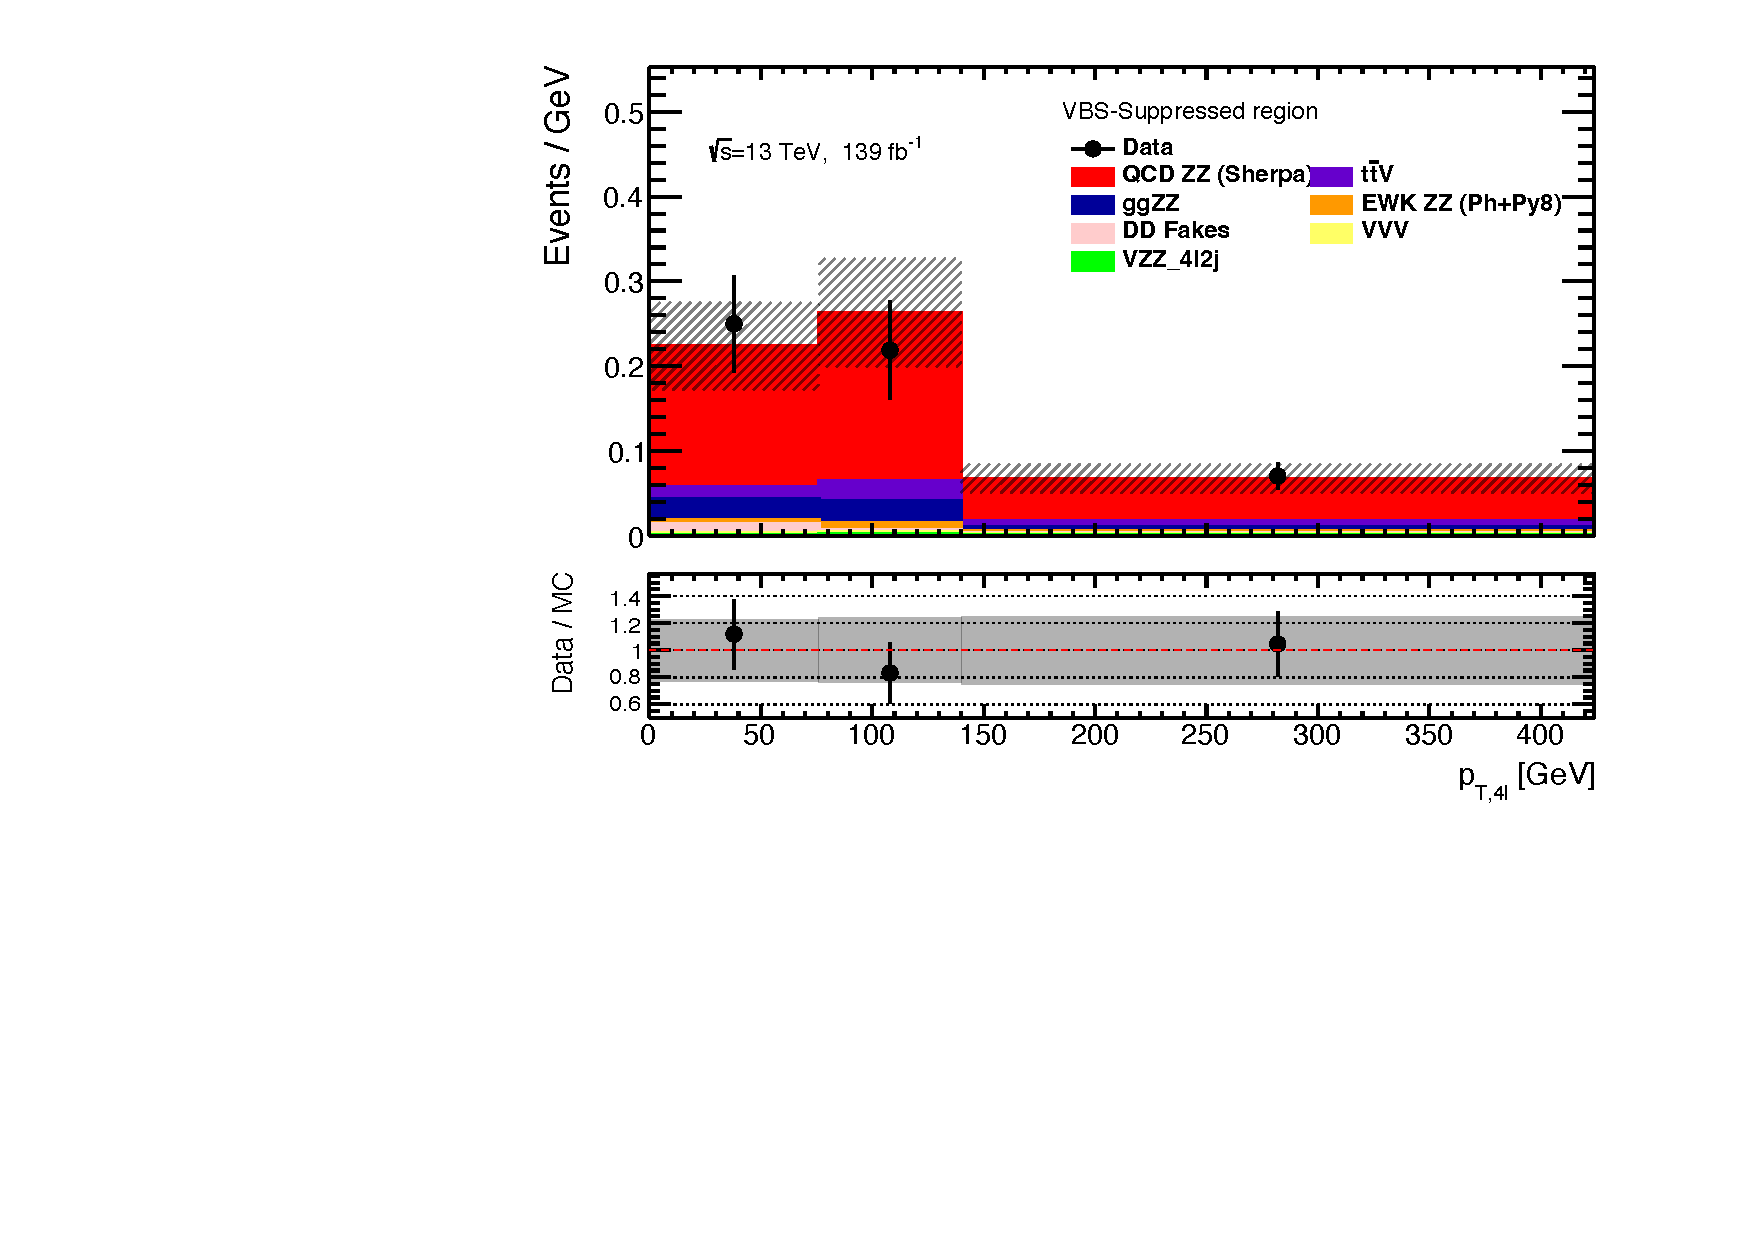
\includegraphics[width=.98\linewidth]{figures/Results/RecoDist_VBSSuppressed/reco_pt4l_CR.pdf}
        \caption{ \footnotesize{$p_{T,4\ell}$ }: $\chi^2/NDF = 0.20$ }
    \end{subfigure}\\
    \begin{subfigure}{.49\textwidth}
        \centering
        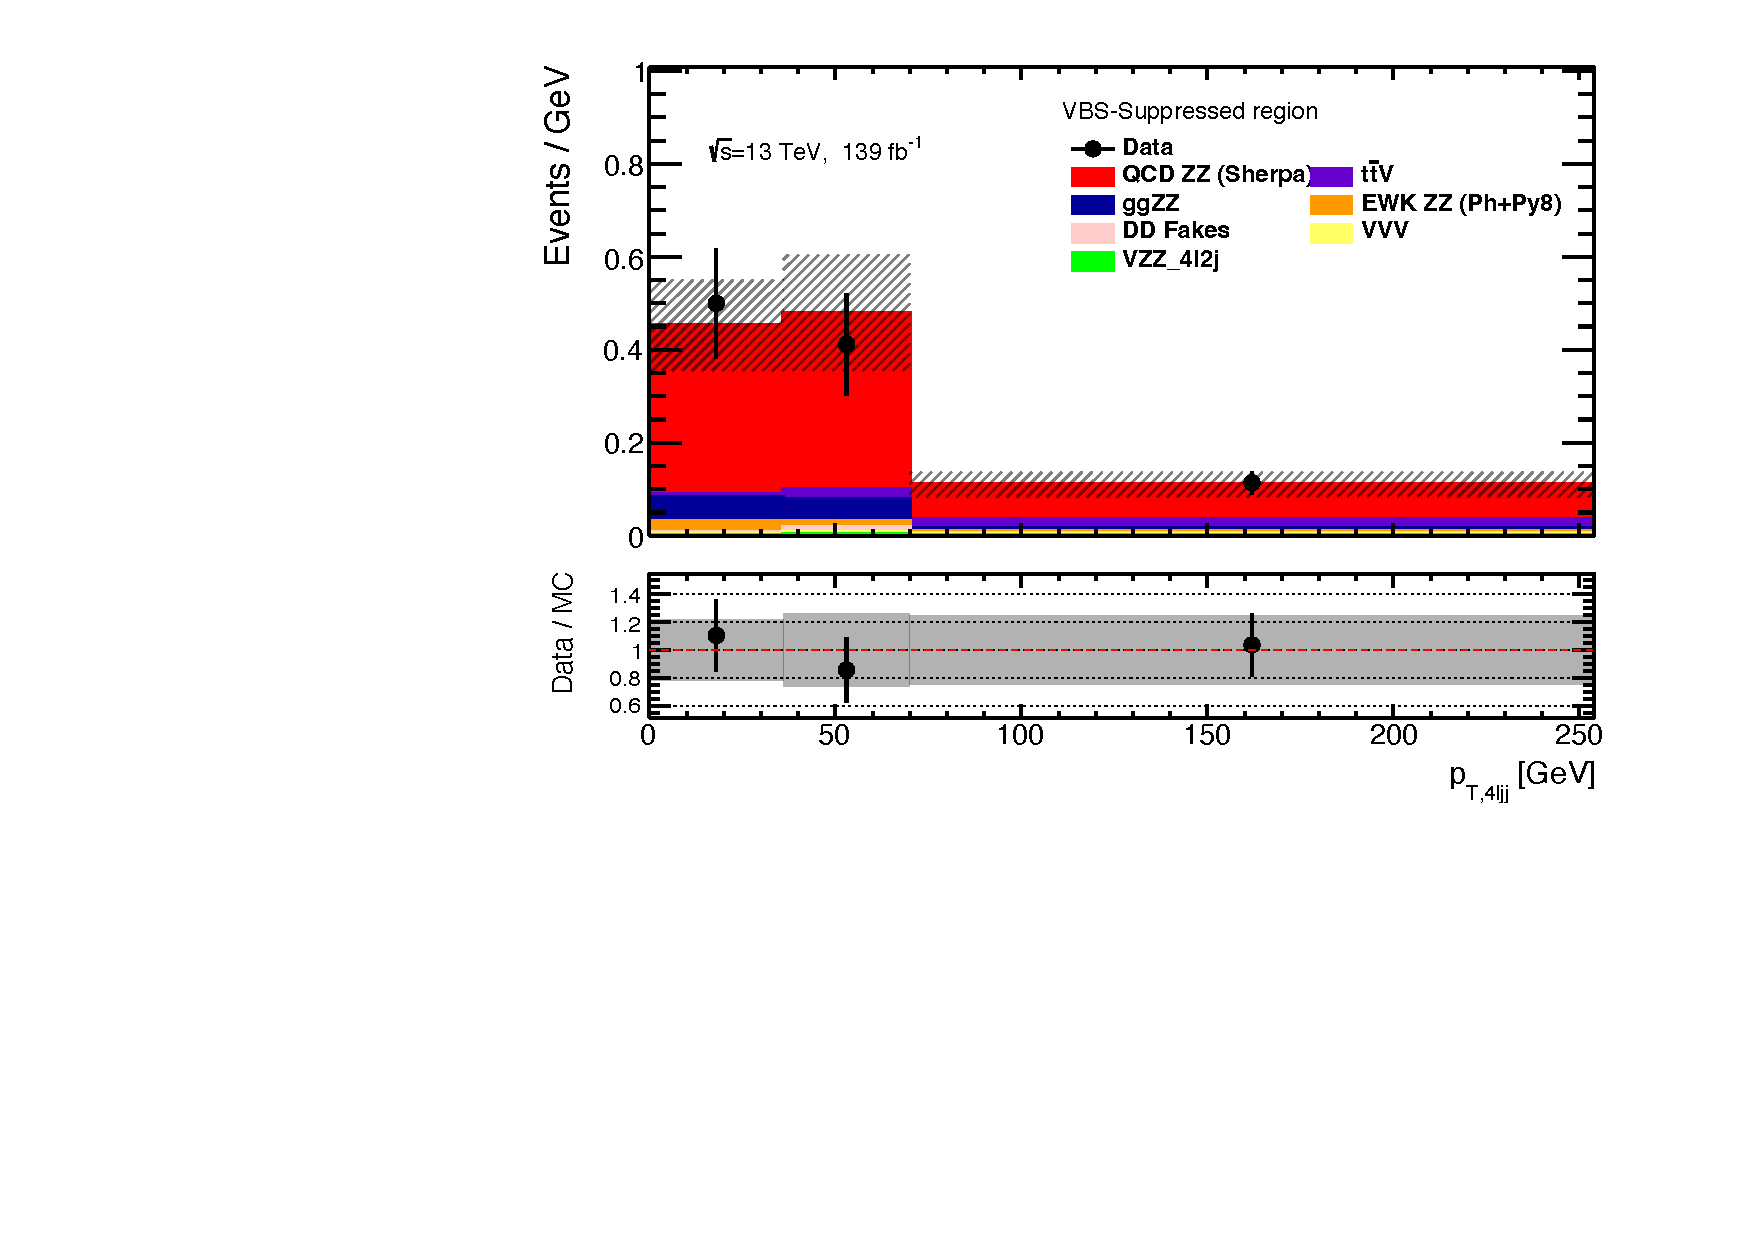
\includegraphics[width=.98\linewidth]{figures/Results/RecoDist_VBSSuppressed/reco_ptzzjj_CR.pdf}
        \caption{ \footnotesize{$p_{T,4\ell jj}$}: $\chi^2/NDF = 0.15$ }
    \end{subfigure}
    \begin{subfigure}{.49\textwidth}
        \centering
        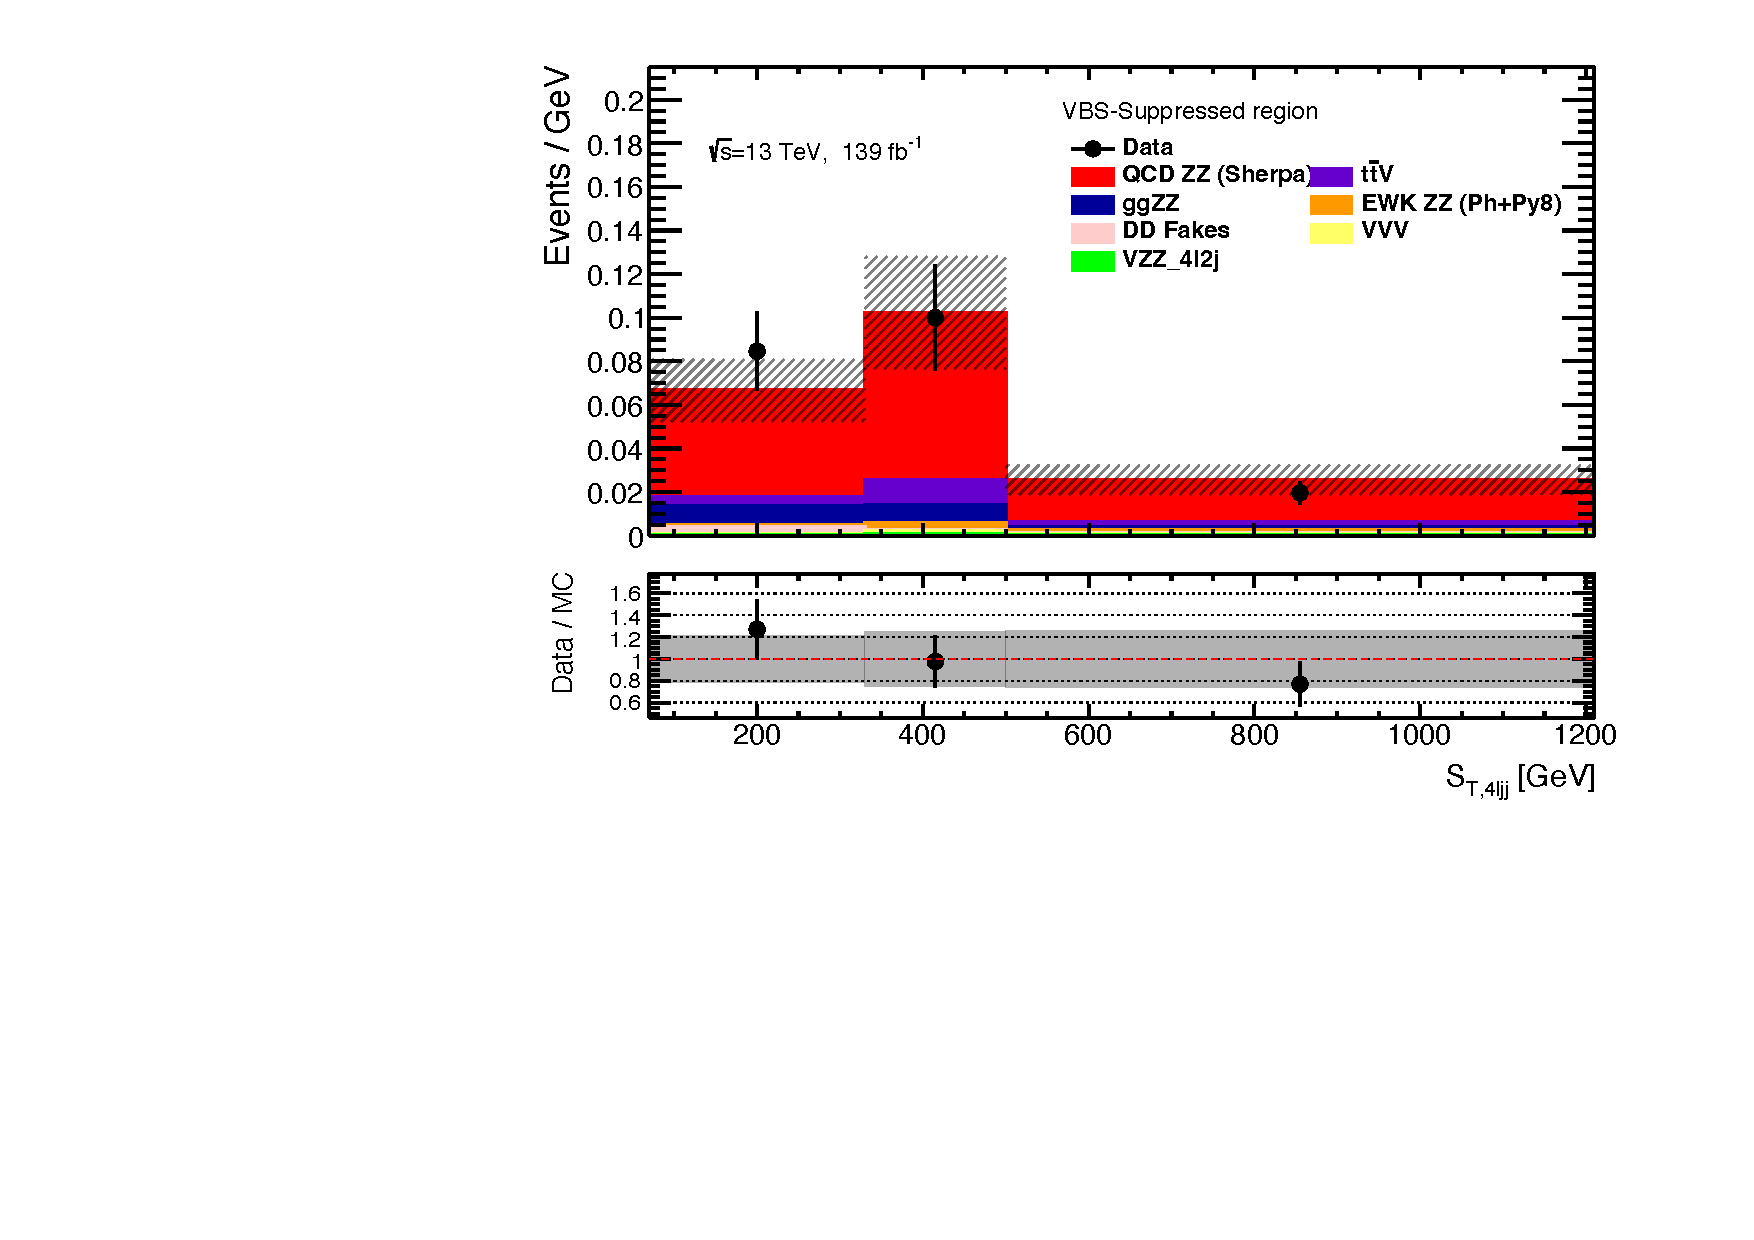
\includegraphics[width=.98\linewidth]{figures/Results/RecoDist_VBSSuppressed/reco_stzzjj_CR.pdf}
        \caption{ \footnotesize{$s_{T, 4\ell jj}$ }: $\chi^2/NDF = 0.58$ }
    \end{subfigure}
    \caption{Detector level distributions in the VBS-Suppressed region.}  \label{fig:reco_VBS_Suppressed_a}
\end{figure}

\begin{figure}[!htb]
    \centering
    \begin{subfigure}{.49\textwidth}
        \centering
        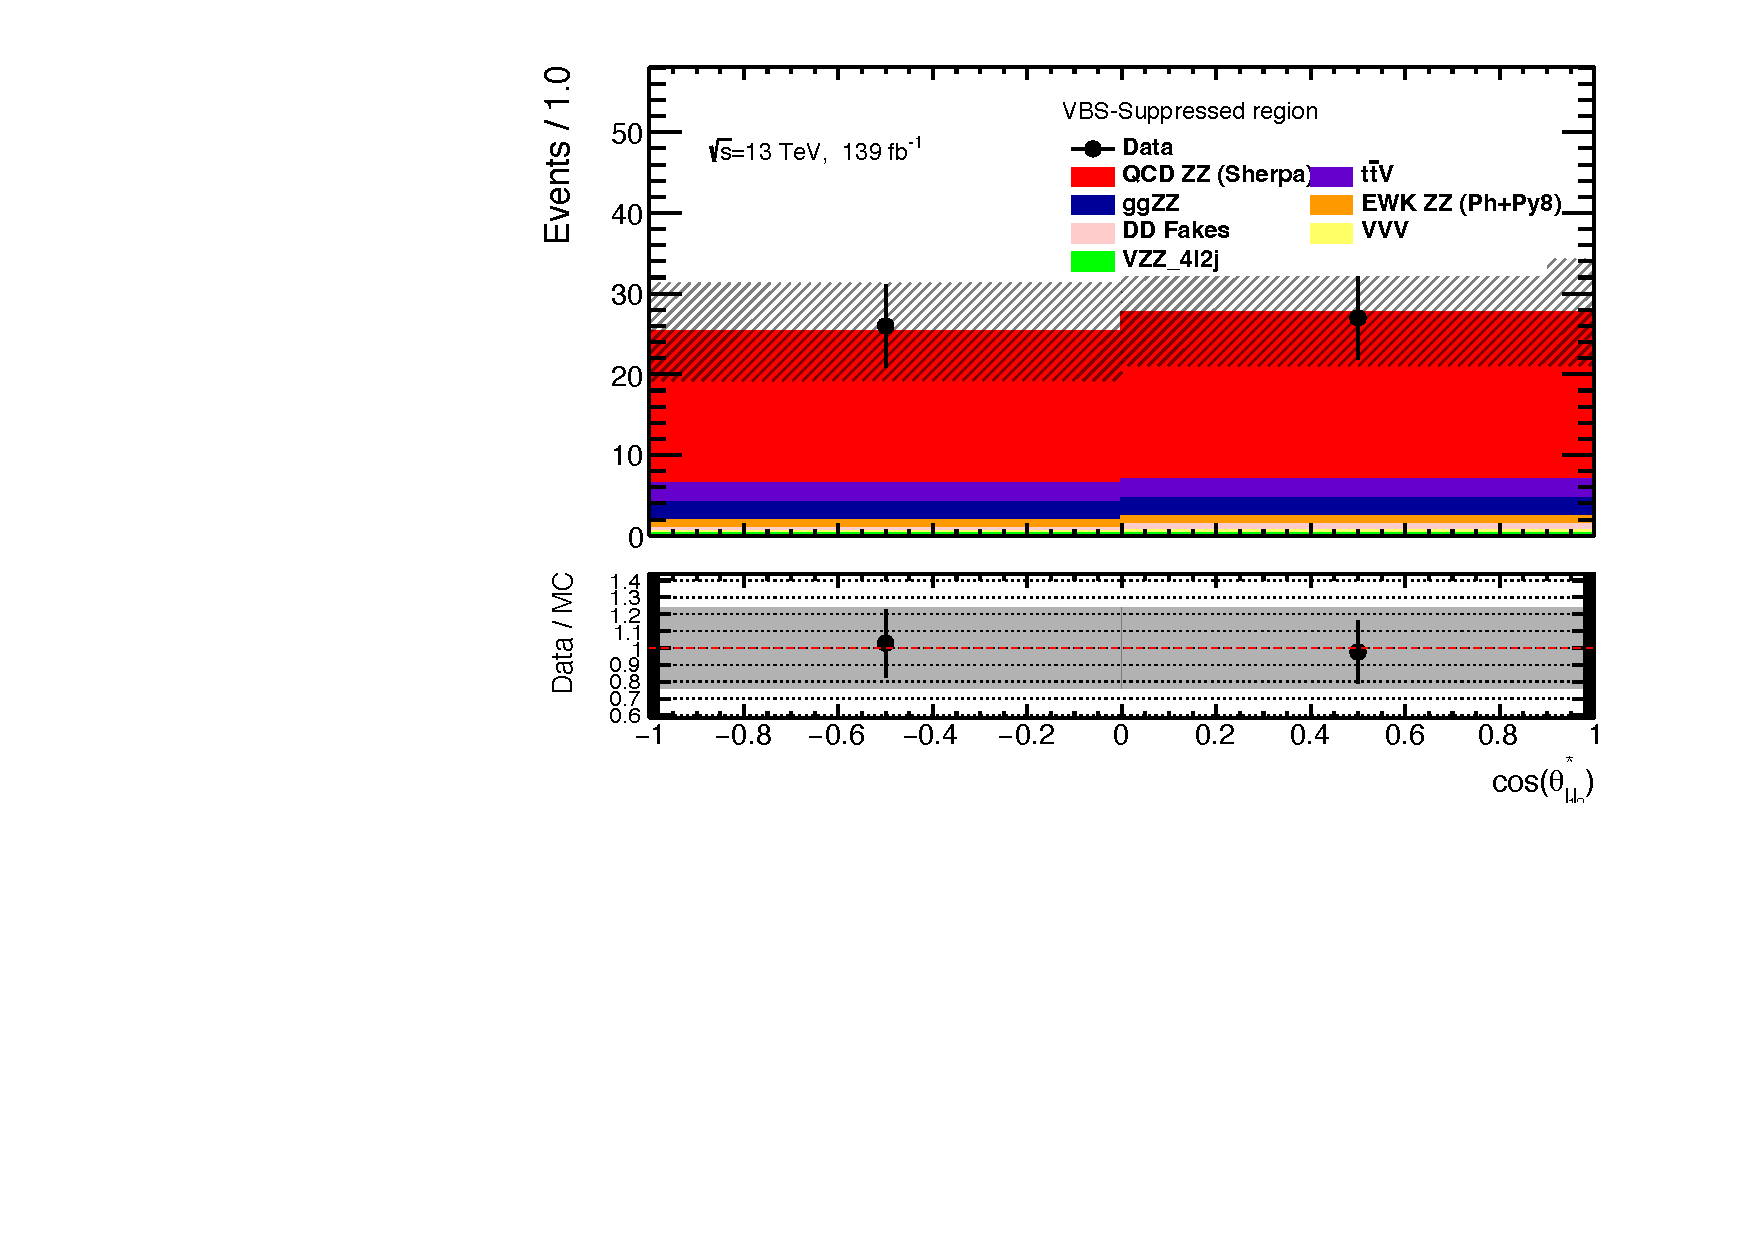
\includegraphics[width=.98\linewidth]{figures/Results/RecoDist_VBSSuppressed/reco_cosThetaStar1_CR.pdf}
        \caption{ \footnotesize{$\cos \theta^{*}_{\ell 1 \ell 2}$}: $\chi^2/NDF = 0.01$ }
    \end{subfigure}
    \begin{subfigure}{.49\textwidth}
        \centering
        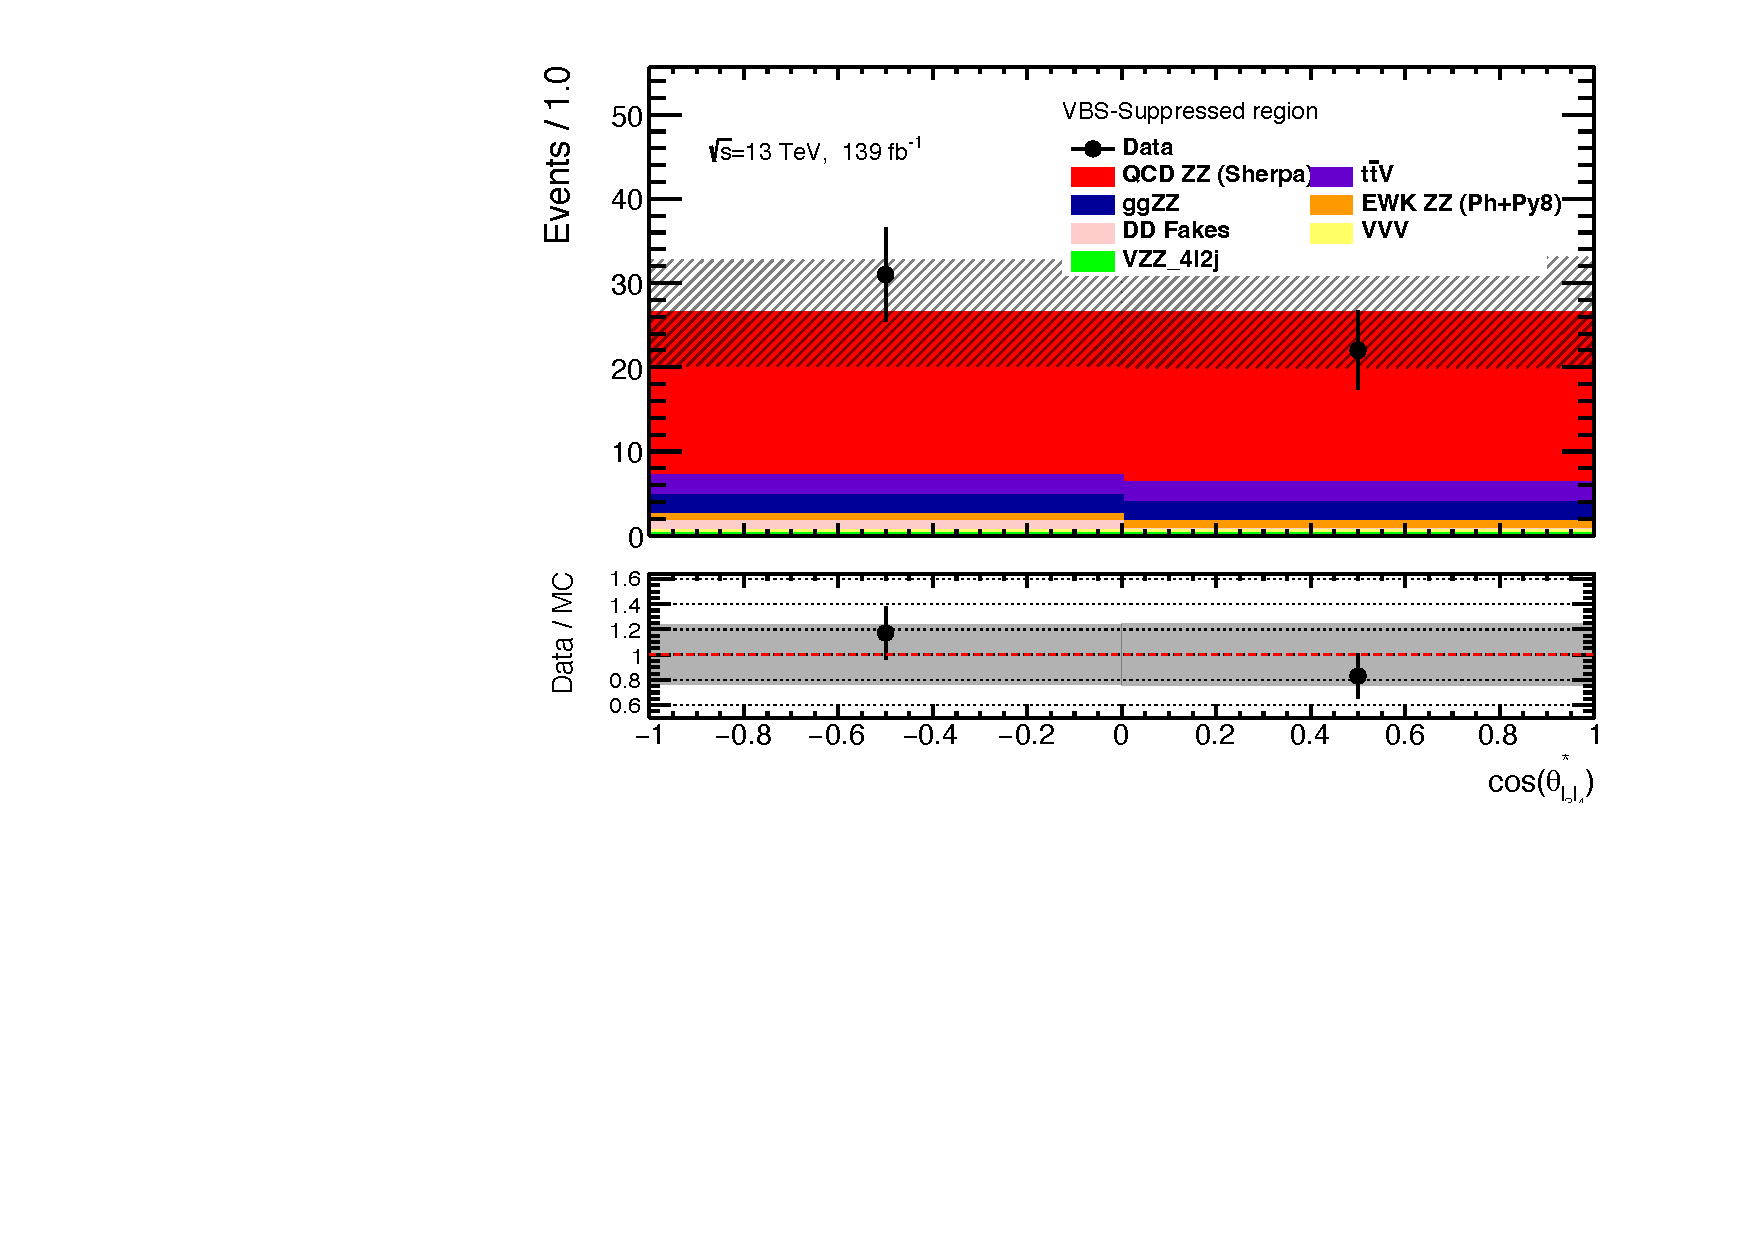
\includegraphics[width=.98\linewidth]{figures/Results/RecoDist_VBSSuppressed/reco_cosThetaStar3_CR.pdf}
        \caption{ \footnotesize{$\cos \theta^{*}_{\ell 3 \ell 4}$ }: $\chi^2/NDF = 0.60$ }
    \end{subfigure}\\
    \begin{subfigure}{.49\textwidth}
        \centering
        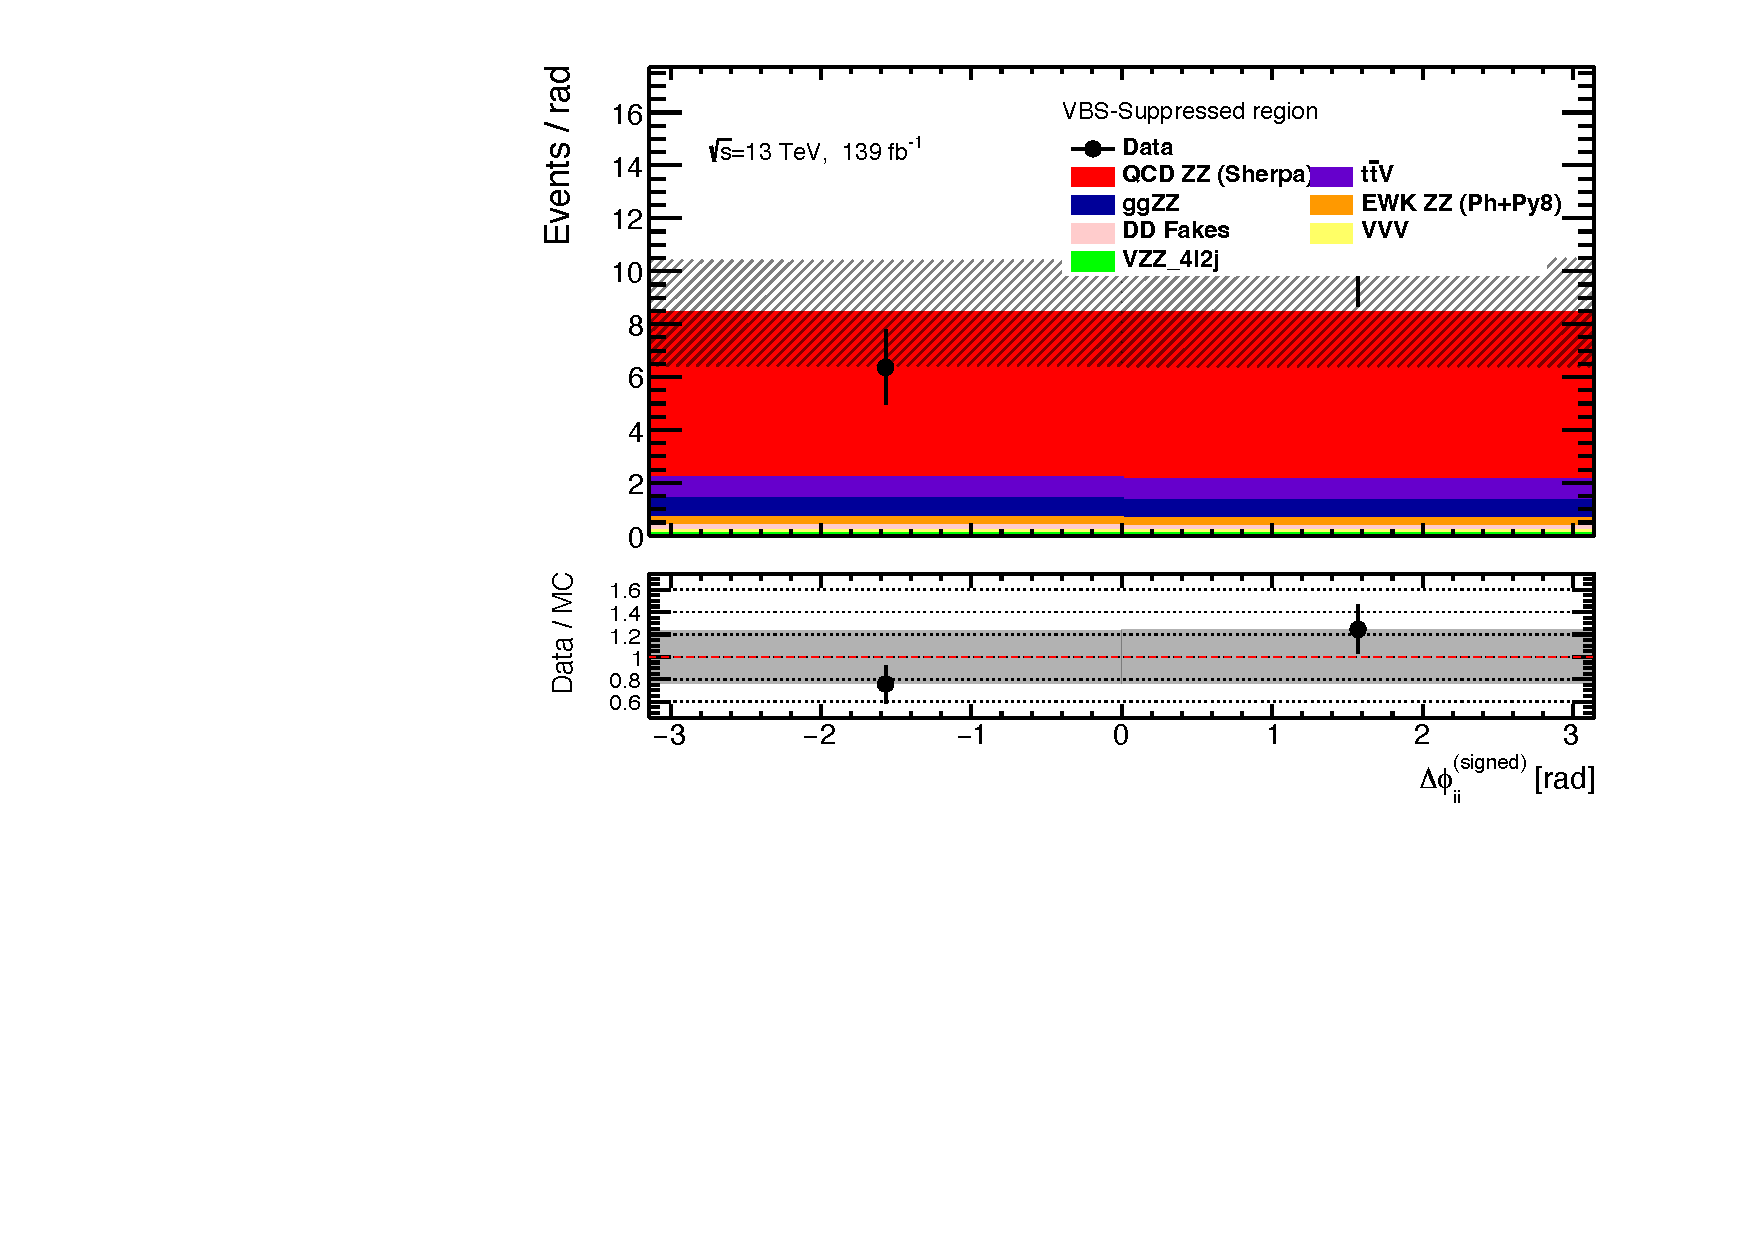
\includegraphics[width=.98\linewidth]{figures/Results/RecoDist_VBSSuppressed/reco_dphi_CR.pdf}
        \caption{ \footnotesize{$\Delta \phi _{jj}^{signed}$ }: $\chi^2/NDF = 1.26$ }
    \end{subfigure}
    \begin{subfigure}{.49\textwidth}
        \centering
        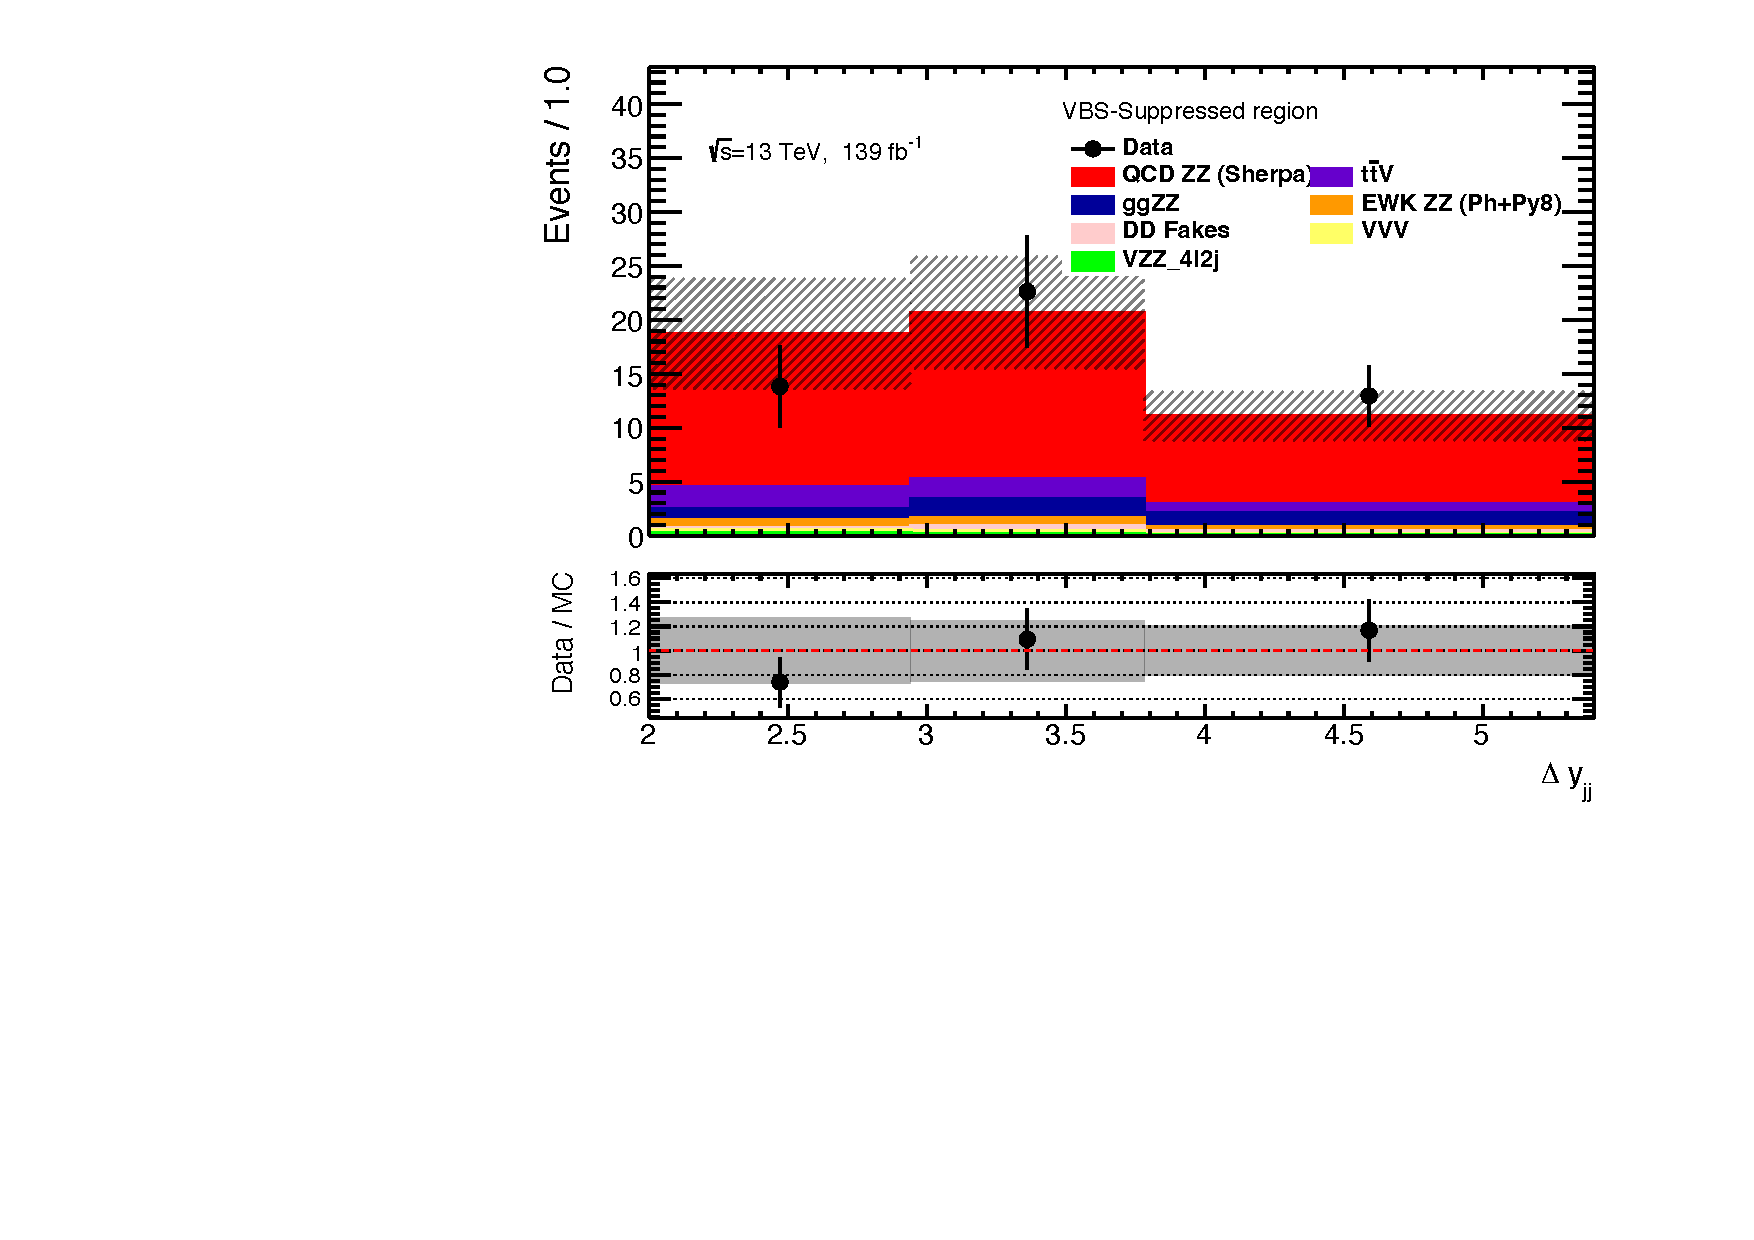
\includegraphics[width=.98\linewidth]{figures/Results/RecoDist_VBSSuppressed/reco_dy_CR.pdf}
        \caption{ \footnotesize{$\Delta y_{jj}$ }: $\chi^2/NDF = 0.55$ }
    \end{subfigure}\\
    \begin{subfigure}{.49\textwidth}
        \centering
        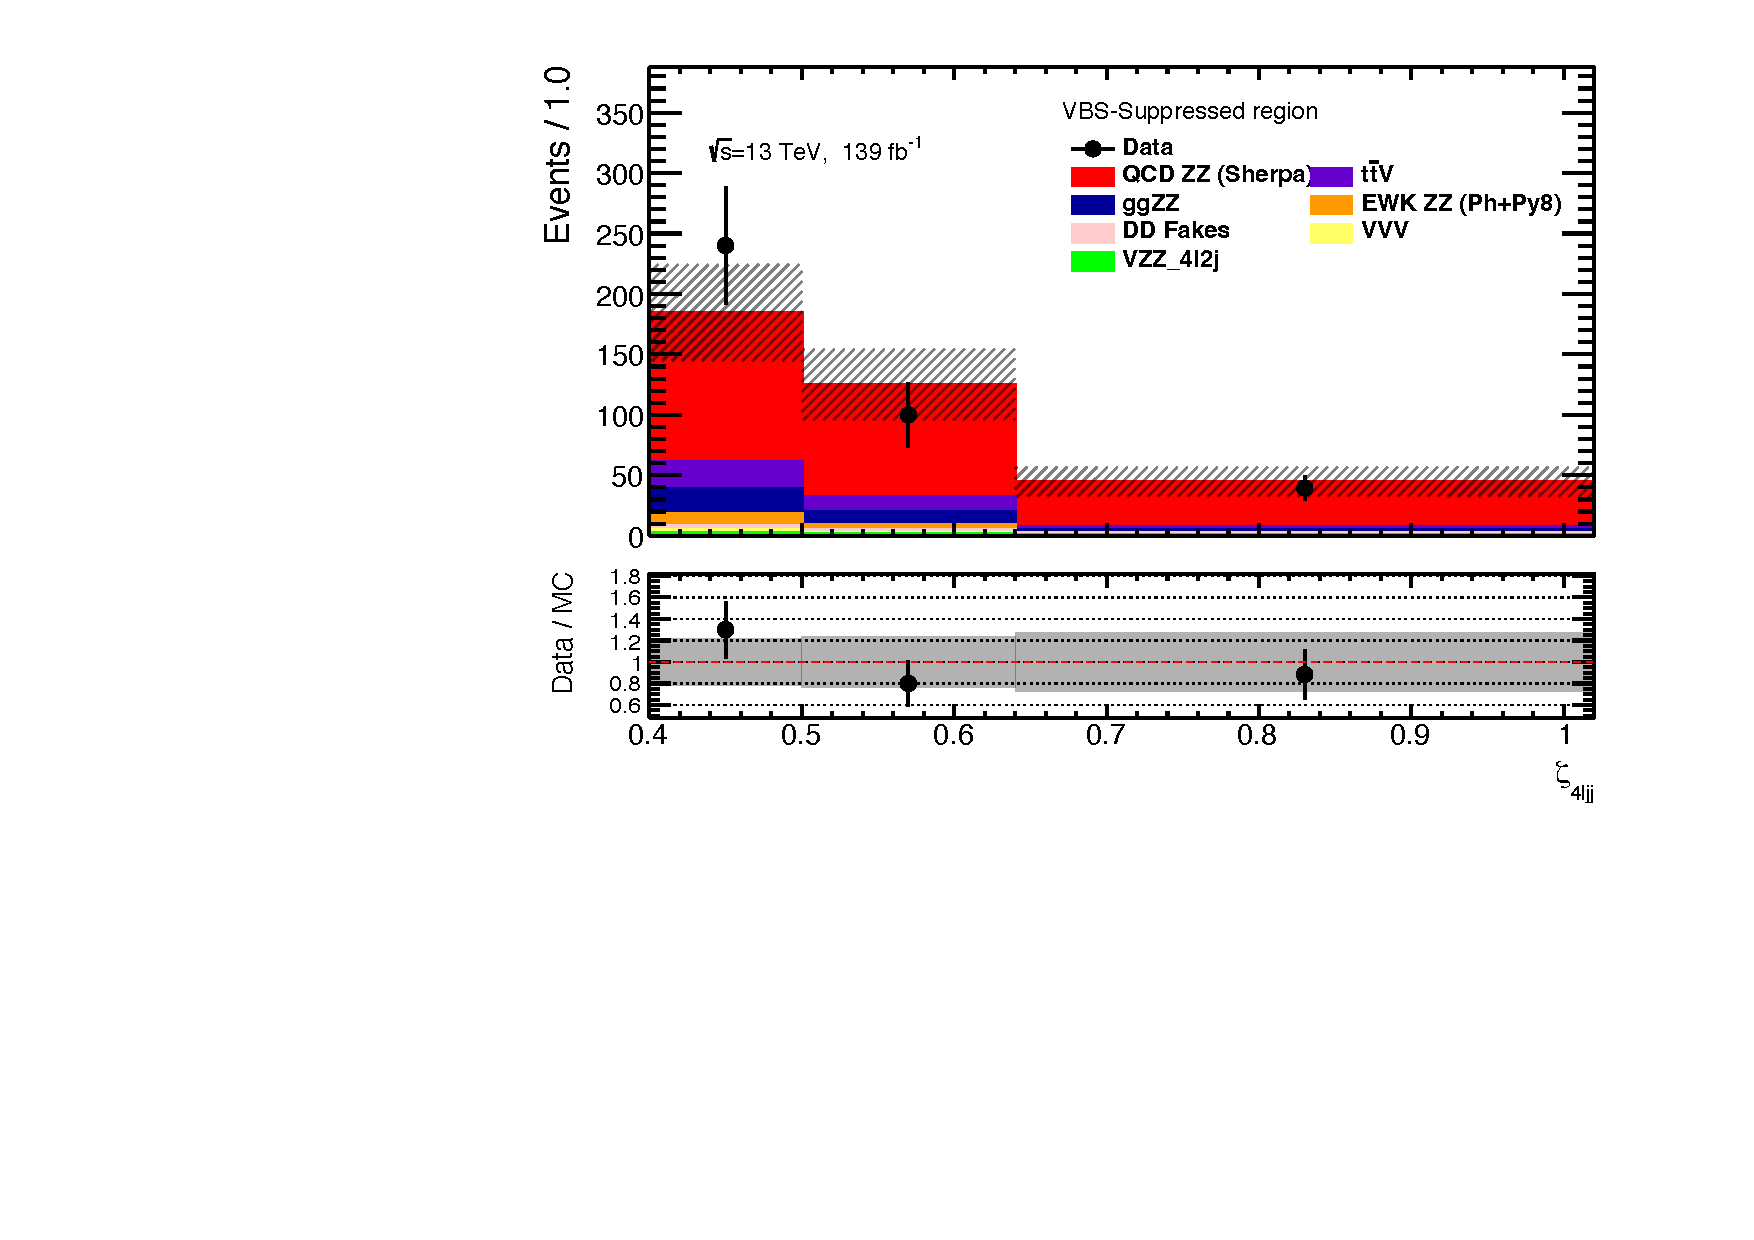
\includegraphics[width=.98\linewidth]{figures/Results/RecoDist_VBSSuppressed/reco_centrality_CR.pdf}
        \caption{ \footnotesize{$\zeta$ }: $\chi^2/NDF = 0.60$ }
    \end{subfigure}
    \caption{Detector level distributions in the VBS-Suppressed region.}  \label{fig:reco_VBS_Suppressed_b}
\end{figure}

\subsection{Unfolded Cross-sections}
\label{appendix:VBSSupUnfolded}

Figures \ref{fig:unfolded_xs_VBS_Suppressed_a} and \ref{fig:unfolded_xs_VBS_Suppressed_b} show the measured unfolded differential cross-sections as a function of the eleven kinematic observables in the VBS-Suppressed region. The unfolded differential cross-sections (black) are compared with two different state-of-the-art SM particle-level predictions, first, where the QCD $qqZZjj$ is generated by \textsc{Sherpa} (red) and second, where the QCD $qqZZjj$ is generated by \textsc{Madgraph} (blue). The vertical-solid line in the black distribution shows the statistical uncertainty of the unfolded cross-sections, and the black band represents the total systematic uncertainties. Similarly, the dashed-red and dashed-blue bands represent the fiducial uncertainties on the \textsc{Sherpa} and \textsc{Madgraph} particle level yield, respectively. Similar to the VBS-Enhanced region, the p-values comparing the unfolded cross-sections with the two truth level yields are also reported. The p-values larger than $0.05$ and the ratios of particle level yields to the unfolded-data yields suggest no statistical deviations of the differential cross-section from the SM predicted values. Therefore, in the analyzed LHC Run-2 dataset, for the $ZZ (\rightarrow 4) \ell jj$ process, all differential cross-sections in the VBS-Suppressed region are concluded to agree with the SM predictions. 

\begin{figure}[!htb]
    \centering
    \begin{subfigure}{.49\textwidth}
        \centering
        \includegraphics[width=.98\linewidth]{figures/Results/CrossSection_VBSSuppressed/xs_mjj_CR.pdf}
        \caption{ \footnotesize{$m_{jj}$}: p-value(Sherpa=0.15 $\&$ MG=0.08)}
    \end{subfigure}
    \begin{subfigure}{.49\textwidth}
        \centering
        \includegraphics[width=.98\linewidth]{figures/Results/CrossSection_VBSSuppressed/xs_m4l_CR.pdf}
        \caption{ \footnotesize{$m_{4\ell}$ }: p-value(Sherpa=0.40 $\&$ MG=0.15)}
    \end{subfigure}\\
    \begin{subfigure}{.49\textwidth}
        \centering
        \includegraphics[width=.98\linewidth]{figures/Results/CrossSection_VBSSuppressed/xs_ptjj_CR.pdf}
        \caption{ \footnotesize{$p_{T,jj}$}: p-value(Sherpa=0.24 $\&$ MG=0.02)}
    \end{subfigure}
    \begin{subfigure}{.49\textwidth}
        \centering
        \includegraphics[width=.98\linewidth]{figures/Results/CrossSection_VBSSuppressed/xs_pt4l_CR.pdf}
        \caption{ \footnotesize{$p_{T,4\ell}$ }: p-value(Sherpa=0.82 $\&$ MG=0.40)}
    \end{subfigure}\\
    \begin{subfigure}{.49\textwidth}
        \centering
        \includegraphics[width=.98\linewidth]{figures/Results/CrossSection_VBSSuppressed/xs_ptzzjj_CR.pdf}
        \caption{ \footnotesize{$p_{T,4\ell jj}$}: p-value(Sherpa=0.96 $\&$ MG=0.08)}
    \end{subfigure}
    \begin{subfigure}{.49\textwidth}
        \centering
        \includegraphics[width=.98\linewidth]{figures/Results/CrossSection_VBSSuppressed/xs_stzzjj_CR.pdf}
        \caption{ \footnotesize{$s_{T, 4\ell jj}$ }: p-value(Sherpa=0.52 $\&$ MG=0.11)}
    \end{subfigure}
    \caption{Unfolded differential cross-sections in the VBS-Suppressed region.}  \label{fig:unfolded_xs_VBS_Suppressed_a}
\end{figure}

\begin{figure}[!htb]
    \centering
    \begin{subfigure}{.49\textwidth}
        \centering
        \includegraphics[width=.98\linewidth]{figures/Results/CrossSection_VBSSuppressed/xs_cosThetaStar1_CR.pdf}
        \caption{ \footnotesize{$\cos \theta^{*}_{\ell 1 \ell 2}$}: p-value(Sherpa=0.90 $\&$ MG=0.81)}
    \end{subfigure}
    \begin{subfigure}{.49\textwidth}
        \centering
        \includegraphics[width=.98\linewidth]{figures/Results/CrossSection_VBSSuppressed/xs_cosThetaStar3_CR.pdf}
        \caption{ \footnotesize{$\cos \theta^{*}_{\ell 3 \ell 4}$ }: p-value(Sherpa=0.43 $\&$ MG=0.41)}
    \end{subfigure}\\
    \begin{subfigure}{.49\textwidth}
        \centering
        \includegraphics[width=.98\linewidth]{figures/Results/CrossSection_VBSSuppressed/xs_dphi_CR.pdf}
        \caption{ \footnotesize{$\Delta \phi _{jj}^{signed}$ }: p-value(Sherpa=0.26 $\&$ MG=0.02)}
    \end{subfigure}
    \begin{subfigure}{.49\textwidth}
        \centering
        \includegraphics[width=.98\linewidth]{figures/Results/CrossSection_VBSSuppressed/xs_dy_CR.pdf}
        \caption{ \footnotesize{$\Delta y_{jj}$ }: p-value(Sherpa=0.57 $\&$ MG=0.32)}
    \end{subfigure}\\
    \begin{subfigure}{.49\textwidth}
        \centering
        \includegraphics[width=.98\linewidth]{figures/Results/CrossSection_VBSSuppressed/xs_centrality_CR.pdf}
        \caption{ \footnotesize{$\zeta$ }: p-value(Sherpa=0.48 $\&$ MG=0.31)}
    \end{subfigure}
    \caption{Unfolded differential cross-sections in the VBS-Suppressed region.}  \label{fig:unfolded_xs_VBS_Suppressed_b}
\end{figure}